% Options for packages loaded elsewhere
% Options for packages loaded elsewhere
\PassOptionsToPackage{unicode}{hyperref}
\PassOptionsToPackage{hyphens}{url}
\PassOptionsToPackage{dvipsnames,svgnames,x11names}{xcolor}
%
\documentclass[
  letterpaper,
  DIV=11,
  numbers=noendperiod,
  oneside]{scrartcl}
\usepackage{xcolor}
\usepackage[margin=1in]{geometry}
\usepackage{amsmath,amssymb}
\setcounter{secnumdepth}{5}
\usepackage{iftex}
\ifPDFTeX
  \usepackage[T1]{fontenc}
  \usepackage[utf8]{inputenc}
  \usepackage{textcomp} % provide euro and other symbols
\else % if luatex or xetex
  \usepackage{unicode-math} % this also loads fontspec
  \defaultfontfeatures{Scale=MatchLowercase}
  \defaultfontfeatures[\rmfamily]{Ligatures=TeX,Scale=1}
\fi
\usepackage{lmodern}
\ifPDFTeX\else
  % xetex/luatex font selection
\fi
% Use upquote if available, for straight quotes in verbatim environments
\IfFileExists{upquote.sty}{\usepackage{upquote}}{}
\IfFileExists{microtype.sty}{% use microtype if available
  \usepackage[]{microtype}
  \UseMicrotypeSet[protrusion]{basicmath} % disable protrusion for tt fonts
}{}
\makeatletter
\@ifundefined{KOMAClassName}{% if non-KOMA class
  \IfFileExists{parskip.sty}{%
    \usepackage{parskip}
  }{% else
    \setlength{\parindent}{0pt}
    \setlength{\parskip}{6pt plus 2pt minus 1pt}}
}{% if KOMA class
  \KOMAoptions{parskip=half}}
\makeatother
% Make \paragraph and \subparagraph free-standing
\makeatletter
\ifx\paragraph\undefined\else
  \let\oldparagraph\paragraph
  \renewcommand{\paragraph}{
    \@ifstar
      \xxxParagraphStar
      \xxxParagraphNoStar
  }
  \newcommand{\xxxParagraphStar}[1]{\oldparagraph*{#1}\mbox{}}
  \newcommand{\xxxParagraphNoStar}[1]{\oldparagraph{#1}\mbox{}}
\fi
\ifx\subparagraph\undefined\else
  \let\oldsubparagraph\subparagraph
  \renewcommand{\subparagraph}{
    \@ifstar
      \xxxSubParagraphStar
      \xxxSubParagraphNoStar
  }
  \newcommand{\xxxSubParagraphStar}[1]{\oldsubparagraph*{#1}\mbox{}}
  \newcommand{\xxxSubParagraphNoStar}[1]{\oldsubparagraph{#1}\mbox{}}
\fi
\makeatother

\usepackage{color}
\usepackage{fancyvrb}
\newcommand{\VerbBar}{|}
\newcommand{\VERB}{\Verb[commandchars=\\\{\}]}
\DefineVerbatimEnvironment{Highlighting}{Verbatim}{commandchars=\\\{\}}
% Add ',fontsize=\small' for more characters per line
\usepackage{framed}
\definecolor{shadecolor}{RGB}{241,243,245}
\newenvironment{Shaded}{\begin{snugshade}}{\end{snugshade}}
\newcommand{\AlertTok}[1]{\textcolor[rgb]{0.68,0.00,0.00}{#1}}
\newcommand{\AnnotationTok}[1]{\textcolor[rgb]{0.37,0.37,0.37}{#1}}
\newcommand{\AttributeTok}[1]{\textcolor[rgb]{0.40,0.45,0.13}{#1}}
\newcommand{\BaseNTok}[1]{\textcolor[rgb]{0.68,0.00,0.00}{#1}}
\newcommand{\BuiltInTok}[1]{\textcolor[rgb]{0.00,0.23,0.31}{#1}}
\newcommand{\CharTok}[1]{\textcolor[rgb]{0.13,0.47,0.30}{#1}}
\newcommand{\CommentTok}[1]{\textcolor[rgb]{0.37,0.37,0.37}{#1}}
\newcommand{\CommentVarTok}[1]{\textcolor[rgb]{0.37,0.37,0.37}{\textit{#1}}}
\newcommand{\ConstantTok}[1]{\textcolor[rgb]{0.56,0.35,0.01}{#1}}
\newcommand{\ControlFlowTok}[1]{\textcolor[rgb]{0.00,0.23,0.31}{\textbf{#1}}}
\newcommand{\DataTypeTok}[1]{\textcolor[rgb]{0.68,0.00,0.00}{#1}}
\newcommand{\DecValTok}[1]{\textcolor[rgb]{0.68,0.00,0.00}{#1}}
\newcommand{\DocumentationTok}[1]{\textcolor[rgb]{0.37,0.37,0.37}{\textit{#1}}}
\newcommand{\ErrorTok}[1]{\textcolor[rgb]{0.68,0.00,0.00}{#1}}
\newcommand{\ExtensionTok}[1]{\textcolor[rgb]{0.00,0.23,0.31}{#1}}
\newcommand{\FloatTok}[1]{\textcolor[rgb]{0.68,0.00,0.00}{#1}}
\newcommand{\FunctionTok}[1]{\textcolor[rgb]{0.28,0.35,0.67}{#1}}
\newcommand{\ImportTok}[1]{\textcolor[rgb]{0.00,0.46,0.62}{#1}}
\newcommand{\InformationTok}[1]{\textcolor[rgb]{0.37,0.37,0.37}{#1}}
\newcommand{\KeywordTok}[1]{\textcolor[rgb]{0.00,0.23,0.31}{\textbf{#1}}}
\newcommand{\NormalTok}[1]{\textcolor[rgb]{0.00,0.23,0.31}{#1}}
\newcommand{\OperatorTok}[1]{\textcolor[rgb]{0.37,0.37,0.37}{#1}}
\newcommand{\OtherTok}[1]{\textcolor[rgb]{0.00,0.23,0.31}{#1}}
\newcommand{\PreprocessorTok}[1]{\textcolor[rgb]{0.68,0.00,0.00}{#1}}
\newcommand{\RegionMarkerTok}[1]{\textcolor[rgb]{0.00,0.23,0.31}{#1}}
\newcommand{\SpecialCharTok}[1]{\textcolor[rgb]{0.37,0.37,0.37}{#1}}
\newcommand{\SpecialStringTok}[1]{\textcolor[rgb]{0.13,0.47,0.30}{#1}}
\newcommand{\StringTok}[1]{\textcolor[rgb]{0.13,0.47,0.30}{#1}}
\newcommand{\VariableTok}[1]{\textcolor[rgb]{0.07,0.07,0.07}{#1}}
\newcommand{\VerbatimStringTok}[1]{\textcolor[rgb]{0.13,0.47,0.30}{#1}}
\newcommand{\WarningTok}[1]{\textcolor[rgb]{0.37,0.37,0.37}{\textit{#1}}}

\usepackage{longtable,booktabs,array}
\usepackage{calc} % for calculating minipage widths
% Correct order of tables after \paragraph or \subparagraph
\usepackage{etoolbox}
\makeatletter
\patchcmd\longtable{\par}{\if@noskipsec\mbox{}\fi\par}{}{}
\makeatother
% Allow footnotes in longtable head/foot
\IfFileExists{footnotehyper.sty}{\usepackage{footnotehyper}}{\usepackage{footnote}}
\makesavenoteenv{longtable}
\usepackage{graphicx}
\makeatletter
\newsavebox\pandoc@box
\newcommand*\pandocbounded[1]{% scales image to fit in text height/width
  \sbox\pandoc@box{#1}%
  \Gscale@div\@tempa{\textheight}{\dimexpr\ht\pandoc@box+\dp\pandoc@box\relax}%
  \Gscale@div\@tempb{\linewidth}{\wd\pandoc@box}%
  \ifdim\@tempb\p@<\@tempa\p@\let\@tempa\@tempb\fi% select the smaller of both
  \ifdim\@tempa\p@<\p@\scalebox{\@tempa}{\usebox\pandoc@box}%
  \else\usebox{\pandoc@box}%
  \fi%
}
% Set default figure placement to htbp
\def\fps@figure{htbp}
\makeatother


% definitions for citeproc citations
\NewDocumentCommand\citeproctext{}{}
\NewDocumentCommand\citeproc{mm}{%
  \begingroup\def\citeproctext{#2}\cite{#1}\endgroup}
\makeatletter
 % allow citations to break across lines
 \let\@cite@ofmt\@firstofone
 % avoid brackets around text for \cite:
 \def\@biblabel#1{}
 \def\@cite#1#2{{#1\if@tempswa , #2\fi}}
\makeatother
\newlength{\cslhangindent}
\setlength{\cslhangindent}{1.5em}
\newlength{\csllabelwidth}
\setlength{\csllabelwidth}{3em}
\newenvironment{CSLReferences}[2] % #1 hanging-indent, #2 entry-spacing
 {\begin{list}{}{%
  \setlength{\itemindent}{0pt}
  \setlength{\leftmargin}{0pt}
  \setlength{\parsep}{0pt}
  % turn on hanging indent if param 1 is 1
  \ifodd #1
   \setlength{\leftmargin}{\cslhangindent}
   \setlength{\itemindent}{-1\cslhangindent}
  \fi
  % set entry spacing
  \setlength{\itemsep}{#2\baselineskip}}}
 {\end{list}}
\usepackage{calc}
\newcommand{\CSLBlock}[1]{\hfill\break\parbox[t]{\linewidth}{\strut\ignorespaces#1\strut}}
\newcommand{\CSLLeftMargin}[1]{\parbox[t]{\csllabelwidth}{\strut#1\strut}}
\newcommand{\CSLRightInline}[1]{\parbox[t]{\linewidth - \csllabelwidth}{\strut#1\strut}}
\newcommand{\CSLIndent}[1]{\hspace{\cslhangindent}#1}



\setlength{\emergencystretch}{3em} % prevent overfull lines

\providecommand{\tightlist}{%
  \setlength{\itemsep}{0pt}\setlength{\parskip}{0pt}}



 


\usepackage{booktabs}
\usepackage{longtable}
\usepackage{array}
\usepackage{multirow}
\usepackage{wrapfig}
\usepackage{float}
\usepackage{colortbl}
\usepackage{pdflscape}
\usepackage{tabu}
\usepackage{threeparttable}
\usepackage{threeparttablex}
\usepackage[normalem]{ulem}
\usepackage{makecell}
\usepackage{xcolor}
\KOMAoption{captions}{tableheading}
\makeatletter
\@ifpackageloaded{tcolorbox}{}{\usepackage[skins,breakable]{tcolorbox}}
\@ifpackageloaded{fontawesome5}{}{\usepackage{fontawesome5}}
\definecolor{quarto-callout-color}{HTML}{909090}
\definecolor{quarto-callout-note-color}{HTML}{0758E5}
\definecolor{quarto-callout-important-color}{HTML}{CC1914}
\definecolor{quarto-callout-warning-color}{HTML}{EB9113}
\definecolor{quarto-callout-tip-color}{HTML}{00A047}
\definecolor{quarto-callout-caution-color}{HTML}{FC5300}
\definecolor{quarto-callout-color-frame}{HTML}{acacac}
\definecolor{quarto-callout-note-color-frame}{HTML}{4582ec}
\definecolor{quarto-callout-important-color-frame}{HTML}{d9534f}
\definecolor{quarto-callout-warning-color-frame}{HTML}{f0ad4e}
\definecolor{quarto-callout-tip-color-frame}{HTML}{02b875}
\definecolor{quarto-callout-caution-color-frame}{HTML}{fd7e14}
\makeatother
\makeatletter
\@ifpackageloaded{caption}{}{\usepackage{caption}}
\AtBeginDocument{%
\ifdefined\contentsname
  \renewcommand*\contentsname{Table of contents}
\else
  \newcommand\contentsname{Table of contents}
\fi
\ifdefined\listfigurename
  \renewcommand*\listfigurename{List of Figures}
\else
  \newcommand\listfigurename{List of Figures}
\fi
\ifdefined\listtablename
  \renewcommand*\listtablename{List of Tables}
\else
  \newcommand\listtablename{List of Tables}
\fi
\ifdefined\figurename
  \renewcommand*\figurename{Figure}
\else
  \newcommand\figurename{Figure}
\fi
\ifdefined\tablename
  \renewcommand*\tablename{Table}
\else
  \newcommand\tablename{Table}
\fi
}
\@ifpackageloaded{float}{}{\usepackage{float}}
\floatstyle{ruled}
\@ifundefined{c@chapter}{\newfloat{codelisting}{h}{lop}}{\newfloat{codelisting}{h}{lop}[chapter]}
\floatname{codelisting}{Listing}
\newcommand*\listoflistings{\listof{codelisting}{List of Listings}}
\makeatother
\makeatletter
\makeatother
\makeatletter
\@ifpackageloaded{caption}{}{\usepackage{caption}}
\@ifpackageloaded{subcaption}{}{\usepackage{subcaption}}
\makeatother
\makeatletter
\@ifpackageloaded{sidenotes}{}{\usepackage{sidenotes}}
\@ifpackageloaded{marginnote}{}{\usepackage{marginnote}}
\makeatother
\usepackage{bookmark}
\IfFileExists{xurl.sty}{\usepackage{xurl}}{} % add URL line breaks if available
\urlstyle{same}
\hypersetup{
  pdftitle={Report on the use of passive acoustic monitoring for the North Slave Métis Alliance},
  pdfauthor={Alex MacPhail; Orna Phelan},
  colorlinks=true,
  linkcolor={blue},
  filecolor={Maroon},
  citecolor={Blue},
  urlcolor={Blue},
  pdfcreator={LaTeX via pandoc}}


\title{Report on the use of passive acoustic monitoring for the North
Slave Métis Alliance}
\author{Alex MacPhail \and Orna Phelan}
\date{2026-03-25}
\begin{document}
\maketitle

\renewcommand*\contentsname{Table of contents}
{
\hypersetup{linkcolor=}
\setcounter{tocdepth}{3}
\tableofcontents
}

\begin{figure}[H]

{\centering \pandocbounded{\includegraphics[keepaspectratio]{./assets/slavelake.png}}

}

\caption{Forest near Behchoko, NWT.}

\end{figure}%

\section{Abstract}\label{abstract}

The North Slave Métis Alliance deployed Autonomous Recording Units
(ARUs) across 19 locations over three years to characterize the acoustic
community. This project is part of a broader community-based monitoring
initiative under the NSMA Guardianship Program, which incorporates game
cameras, ARUs, water quality sampling, and eDNA to assess biodiversity
in the North Slave Region. A total of 81 species were detected, 4
species-at-risk, with species accumulation beginning to stabilize as
more locations were surveyed. These results highlight the effectiveness
of ARUs in detecting species and their potential to enhance the overall
North Slave species monitoring programs. Continued long-term sampling of
sites already surveyed, along with the inclusion of new locations in
areas that reflect the dynamic northern landscape, is recommended to
sustain and improve monitoring efforts.

\begin{tcolorbox}[enhanced jigsaw, opacitybacktitle=0.6, colframe=quarto-callout-note-color-frame, rightrule=.15mm, coltitle=black, opacityback=0, title=\textcolor{quarto-callout-note-color}{\faInfo}\hspace{0.5em}{Note}, left=2mm, toprule=.15mm, breakable, bottomtitle=1mm, toptitle=1mm, titlerule=0mm, leftrule=.75mm, colback=white, colbacktitle=quarto-callout-note-color!10!white, arc=.35mm, bottomrule=.15mm]

This report is dynamically generated, meaning its results may evolve
with the addition of new data or further analyses. For the most recent
updates, refer to the publication date and feel free to reach out to the
authors.

\end{tcolorbox}

\begin{Shaded}
\begin{Highlighting}[]
\CommentTok{\# Download data from WildTrax}
\NormalTok{nsma\_projects }\OtherTok{\textless{}{-}}\NormalTok{ wildrtrax}\SpecialCharTok{::}\FunctionTok{wt\_get\_projects}\NormalTok{(}\AttributeTok{sensor =} \StringTok{\textquotesingle{}ARU\textquotesingle{}}\NormalTok{) }\SpecialCharTok{|\textgreater{}}
  \FunctionTok{filter}\NormalTok{(}\FunctionTok{grepl}\NormalTok{(}\StringTok{\textquotesingle{}\^{}North Slave\textquotesingle{}}\NormalTok{, project)) }\SpecialCharTok{|\textgreater{}}
  \FunctionTok{select}\NormalTok{(project\_id) }\SpecialCharTok{|\textgreater{}}
  \FunctionTok{pull}\NormalTok{()}

\NormalTok{nsma\_main }\OtherTok{\textless{}{-}}
  \FunctionTok{map\_dfr}\NormalTok{(}
    \AttributeTok{.x =}\NormalTok{ nsma\_projects,}
    \AttributeTok{.f =} \SpecialCharTok{\textasciitilde{}}\NormalTok{ wildrtrax}\SpecialCharTok{::}\FunctionTok{wt\_download\_report}\NormalTok{(}
      \AttributeTok{project\_id =}\NormalTok{ .x,}
      \AttributeTok{sensor\_id =} \StringTok{"ARU"}\NormalTok{,}
      \AttributeTok{reports =} \StringTok{"main"}
\NormalTok{    )}
\NormalTok{  )}
\end{Highlighting}
\end{Shaded}

\section{Land Acknowledgement}\label{land-acknowledgement}

We acknowledge the traditional lands and territories of the North Slave
Métis Alliance (NSMA), whose members trace their origins to the early
unions of French fur-traders and Indigenous women of the Great Slave
Lake region. The Métis of this area have long existed as a distinct and
vibrant community, exercising their harvesting rights across the
Northwest Territories and beyond. We honour their continued stewardship
of these lands and their rights recognized under section 35(1) of the
Constitution Act, 1982.

\section{Introduction}\label{introduction}

Human activities have been identified as key pressures and contributors
to the global decline in forest wildlife (Allan et al. (2017)). The
repercussions of habitat fragmentation (Fahrig (2003)) and loss (Hanski
(2011)), climate change (Mantyka-pringle, Martin, and Rhodes (2012),
Sattar et al. (2021), Abrahms et al. (2023)), and increased access to
sensitive areas exert direct and indirect pressures on forest
biodiversity, particularly in managed regions in Canada (Lemieux et al.
(2011)). Climate change and increasing wildfire activity in the western
and northern boreal have significantly impacted biodiversity and species
interactions in this area. Wildfire severity, intensified by climate
change, significantly influences avian communities in northern boreal
regions, with increasing severity favouring generalist and
fire-specialist species while reducing species richness and functional
diversity in sensitive habitats such as peatlands (Knaggs et al.
(2020)). Furthermore, efforts to use umbrella species, like woodland
caribou, for boreal landbird conservation highlights the need for
complementary conservation measures (Micheletti et al. (2023)) that work
in tandem.

In 2022, the North Slave Métis Alliance initiated a program
incorporating autonomous recording units (ARUs) for passive acoustic
monitoring of the vocalizing wildlife. ARUs are compact environmental
sensors that are designed to passively record the environment (Shonfield
and Bayne (2017)), capturing vocalizing species like birds and
amphibians, which is growing in use across the globe (Sugai et al.
(2018)). This technology enables resource managers to conduct prolonged
surveys with minimal human interference. The subsequent data collected
by these units contribute valuable information to metrics that can be
used to study species trends over time, whereby this data aids
decision-making and management within the region. Given the rapid and
ease of accumulating data from these units, maintaining a high standard
of data integrity is paramount to ensure future data interoperability
and sharing. \href{https://www.wildtrax.ca}{WildTrax} is an online
platform developed by the \href{https://abmi.ca}{Alberta Biodiversity
Monitoring Institute (\textbf{ABMI})} for users of environmental sensors
to help addresses these big data challenges by providing solutions to
standardize, harmonize, and share data.

The report summarizes the data collected from the ARUs by the NSMA from
2022 to 2024. To enhance accessibility and reproducibility, the findings
will be presented in this online report with fully documented code,
allowing future updates as data collection methods become standardized.
Additionally, recommendations will be developed to refine data
transcription priorities, improve annual reporting methods, and evaluate
recommendations for long-term monitoring. The objectives of this report
are to:

\begin{itemize}
\tightlist
\item
  Document and standardize the data management and processing procedures
  for acoustic data collected to ensure consistency and reproducibility.
\item
  Provide a comprehensive report detailing all detected species and the
  abundance of individuals within the surveyed area.
\item
  Facilitate the publication of data, making it accessible to the
  community, public, resource managers, academic institutions, and other
  relevant agencies to promote transparency and collaboration.
\item
  Use evaluation results to establish robust metrics that can inform
  long-term monitoring and conservation strategies.
\end{itemize}

\section{Methods}\label{methods}

\subsection{Data collection}\label{data-collection}

Survey site selection was guided by the goal of capturing a
representative sample of the region's diverse habitats while considering
logistical feasibility. In addition, NSMA member's Traditional Knowledge
of the land and historical distribution of species-at-risk was
incorporated into the study design. Several NSMA members were
interviewed and asked to identify areas of interest for sampling based
on the following criteria:

\begin{enumerate}
\def\labelenumi{\arabic{enumi}.}
\tightlist
\item
  Current or historical presence of the target species at risk in the
  North Slave region;
\item
  Locations of importance to traditional harvesting of NSMA membership,
  and,
\item
  Locations where multiple species, species-at-risk (SAR) or non-SAR,
  are present
\end{enumerate}

Locations were all located within the Taiga Shield Ecozone, encompassing
a heterogeneous landscape of upland forests, wetlands, peatlands, and
freshwater systems. Sampling locations were strategically distributed to
maximize coverage across these habitat types while also sampling areas
of importance to NSMA members. Detailed coordinates and descriptions of
the sampling locations are provided in Table~\ref{tbl-loc-summary}. ARUs
were deployed over three consecutive years (2022, 2023, and 2024); in
2022, two locations were surveyed at Old Fort Rae (62.65084, -115.8187;
62.64749, -115.8198). The survey expanded in 2023 to include eight
locations spanning a larger geographic area, from Whatì (63.10753,
-116.9763) to Tibbitt Lake (62.5474, -113.3551). In 2024, four
additional sites were added to the original eight, increasing the total
to twelve locations and enhancing spatial coverage. ARUs were deployed
at each site to continuously record the soundscape, allowing for the
analysis of acoustic activity patterns and species presence across the
study area.

\begin{Shaded}
\begin{Highlighting}[]
\NormalTok{nsma\_locs }\OtherTok{\textless{}{-}}\NormalTok{ nsma\_main }\SpecialCharTok{|\textgreater{}}
  \FunctionTok{mutate}\NormalTok{(}\AttributeTok{year =}\NormalTok{ lubridate}\SpecialCharTok{::}\FunctionTok{year}\NormalTok{(recording\_date\_time)) }\SpecialCharTok{|\textgreater{}}
  \FunctionTok{select}\NormalTok{(location, latitude, longitude, year) }\SpecialCharTok{|\textgreater{}}
  \FunctionTok{distinct}\NormalTok{() }\SpecialCharTok{|\textgreater{}}
  \FunctionTok{drop\_na}\NormalTok{(latitude) }\SpecialCharTok{|\textgreater{}}
\NormalTok{  sf}\SpecialCharTok{::}\FunctionTok{st\_as\_sf}\NormalTok{(}\AttributeTok{coords =} \FunctionTok{c}\NormalTok{(}\StringTok{"longitude"}\NormalTok{,}\StringTok{"latitude"}\NormalTok{), }\AttributeTok{crs =} \DecValTok{4326}\NormalTok{)}

\NormalTok{locs\_summary }\OtherTok{\textless{}{-}}\NormalTok{ nsma\_locs }\SpecialCharTok{|\textgreater{}}
  \FunctionTok{st\_drop\_geometry}\NormalTok{() }\SpecialCharTok{|\textgreater{}}
  \FunctionTok{group\_by}\NormalTok{(location, year) }\SpecialCharTok{|\textgreater{}}
  \FunctionTok{mutate}\NormalTok{(}\AttributeTok{value =} \FunctionTok{row\_number}\NormalTok{()) }\SpecialCharTok{|\textgreater{}}
  \FunctionTok{ungroup}\NormalTok{() }\SpecialCharTok{|\textgreater{}}
  \FunctionTok{arrange}\NormalTok{(year) }\SpecialCharTok{|\textgreater{}}
  \FunctionTok{pivot\_wider}\NormalTok{(}\AttributeTok{names\_from =}\NormalTok{ year, }\AttributeTok{values\_from =}\NormalTok{ value, }\AttributeTok{values\_fill =} \DecValTok{0}\NormalTok{) }\SpecialCharTok{|\textgreater{}}
  \FunctionTok{inner\_join}\NormalTok{(nsma\_main }\SpecialCharTok{|\textgreater{}} \FunctionTok{select}\NormalTok{(location, latitude, longitude) }\SpecialCharTok{|\textgreater{}} \FunctionTok{distinct}\NormalTok{(), }\AttributeTok{by =} \StringTok{"location"}\NormalTok{) }\SpecialCharTok{|\textgreater{}}
  \FunctionTok{rename}\NormalTok{(}\StringTok{\textquotesingle{}Location\textquotesingle{}} \OtherTok{=}\NormalTok{ location) }\SpecialCharTok{|\textgreater{}}
  \FunctionTok{relocate}\NormalTok{(}\FunctionTok{c}\NormalTok{(latitude, longitude), }\AttributeTok{.after =}\NormalTok{ Location)}

\NormalTok{years }\OtherTok{\textless{}{-}} \DecValTok{2022}\SpecialCharTok{:}\DecValTok{2025}
\NormalTok{colors }\OtherTok{\textless{}{-}} \FunctionTok{c}\NormalTok{(}\StringTok{"yellow"}\NormalTok{, }\StringTok{"blue"}\NormalTok{, }\StringTok{"red"}\NormalTok{, }\StringTok{"green"}\NormalTok{)}
\NormalTok{color\_map }\OtherTok{\textless{}{-}} \FunctionTok{setNames}\NormalTok{(colors, years)}

\NormalTok{base\_map }\OtherTok{\textless{}{-}} \FunctionTok{leaflet}\NormalTok{() }\SpecialCharTok{\%\textgreater{}\%} \FunctionTok{addTiles}\NormalTok{()}

\NormalTok{map }\OtherTok{\textless{}{-}}\NormalTok{ purrr}\SpecialCharTok{::}\FunctionTok{reduce}\NormalTok{(years, }\ControlFlowTok{function}\NormalTok{(map, yr) \{}
\NormalTok{  data }\OtherTok{\textless{}{-}}\NormalTok{ nsma\_locs }\SpecialCharTok{|\textgreater{}} \FunctionTok{filter}\NormalTok{(year }\SpecialCharTok{==}\NormalTok{ yr)}
\NormalTok{  map }\SpecialCharTok{|\textgreater{}} \FunctionTok{addCircleMarkers}\NormalTok{(}
    \AttributeTok{data =}\NormalTok{ data,}
    \AttributeTok{color =}\NormalTok{ color\_map[[}\FunctionTok{as.character}\NormalTok{(yr)]],}
    \AttributeTok{group =} \FunctionTok{paste0}\NormalTok{(yr, }\StringTok{" Locations"}\NormalTok{),}
    \AttributeTok{popup =} \SpecialCharTok{\textasciitilde{}}\FunctionTok{paste}\NormalTok{(}\StringTok{"Location:"}\NormalTok{, location)}
\NormalTok{  )\}, }\AttributeTok{.init =}\NormalTok{ base\_map)}

\NormalTok{map }\SpecialCharTok{|\textgreater{}}
  \FunctionTok{addLayersControl}\NormalTok{(}
    \AttributeTok{overlayGroups =} \FunctionTok{paste0}\NormalTok{(years, }\StringTok{" Locations"}\NormalTok{),}
    \AttributeTok{options =} \FunctionTok{layersControlOptions}\NormalTok{(}\AttributeTok{collapsed =} \ConstantTok{FALSE}\NormalTok{)}
\NormalTok{  ) }\SpecialCharTok{|\textgreater{}}
  \FunctionTok{addMeasure}\NormalTok{() }\SpecialCharTok{|\textgreater{}}
  \FunctionTok{addMiniMap}\NormalTok{(}\AttributeTok{position =} \StringTok{"bottomleft"}\NormalTok{)}
\end{Highlighting}
\end{Shaded}

\begin{figure}[H]

\centering{

\pandocbounded{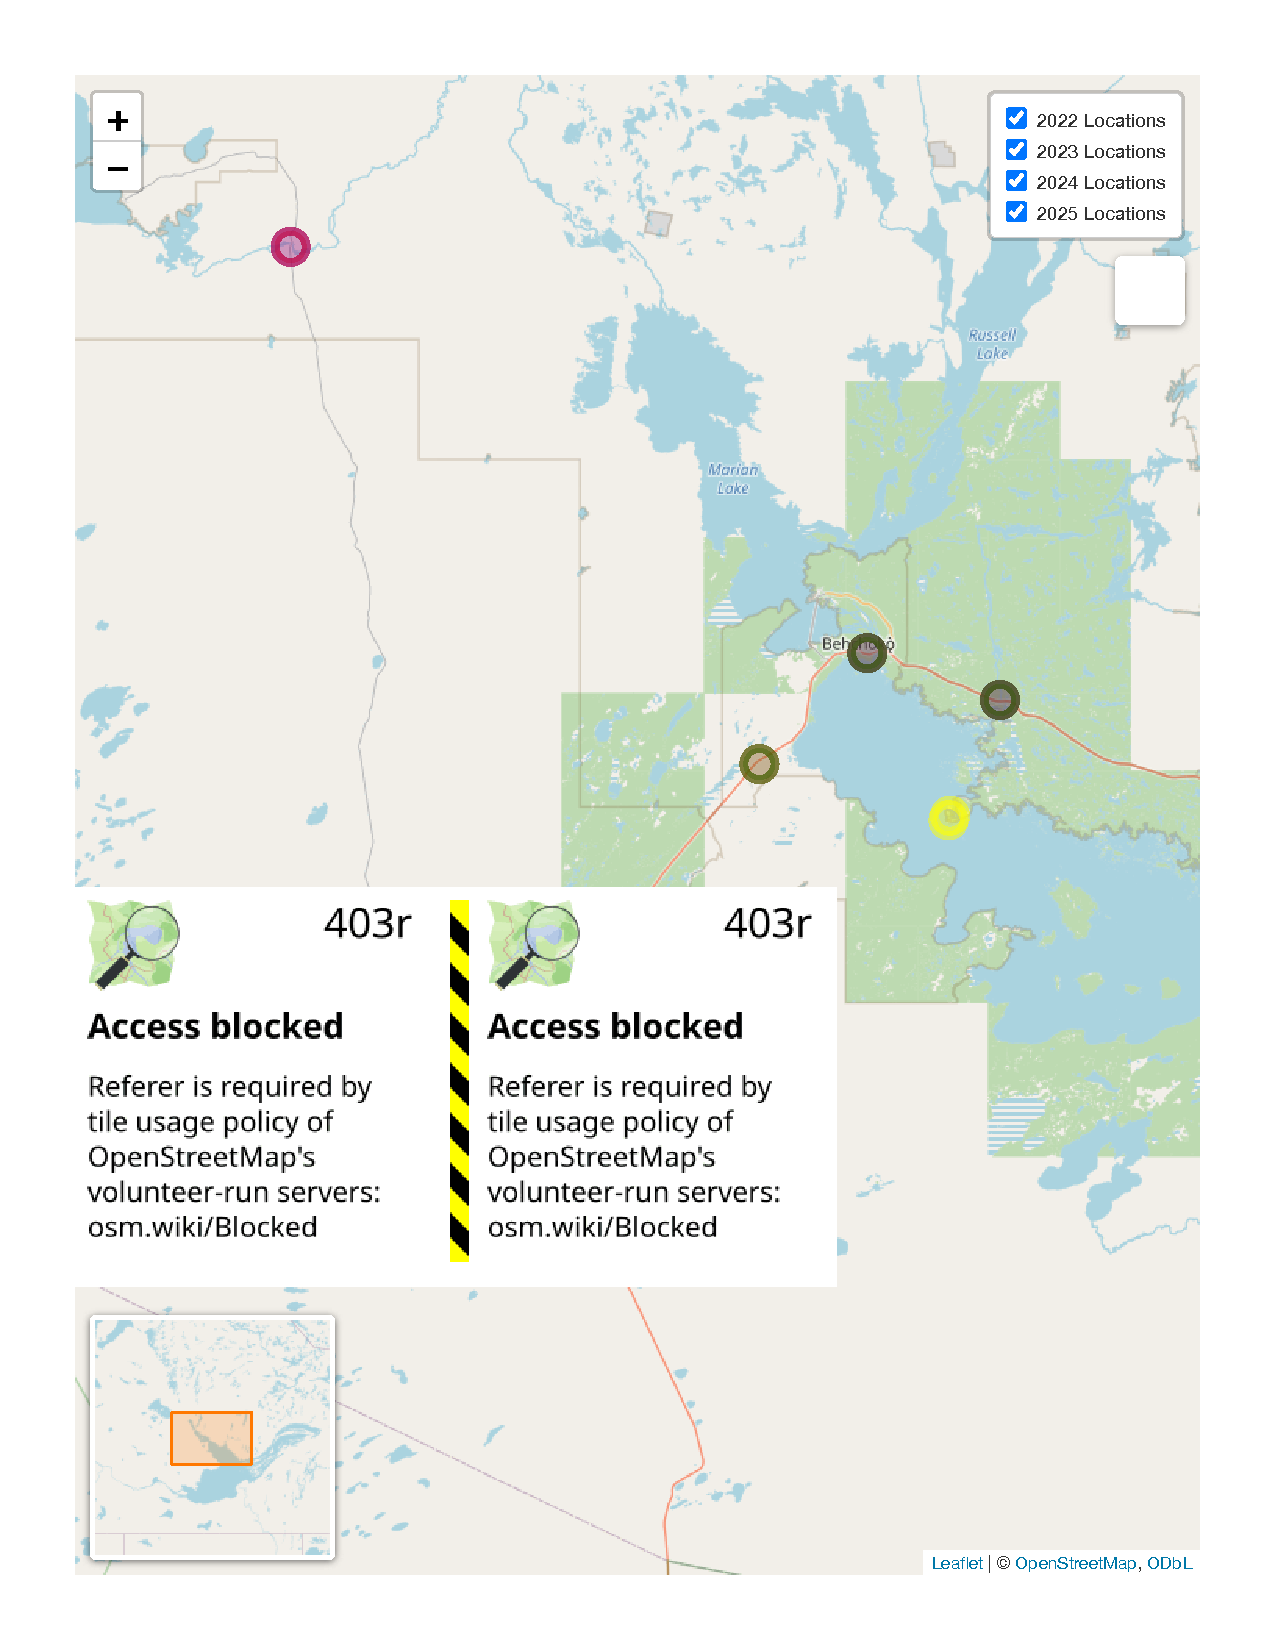
\includegraphics[keepaspectratio]{nsma_files/figure-pdf/fig-aru-monitoring-locations-1.pdf}}

}

\caption{\label{fig-aru-monitoring-locations}Locations from North Slave
Métis Alliance ARU Monitoring Program}

\end{figure}%

\begin{table}

\caption{\label{tbl-loc-summary}Locations surveyed across years. Ones
indicated a deployment in that year for that location.}

\centering{

\pandocbounded{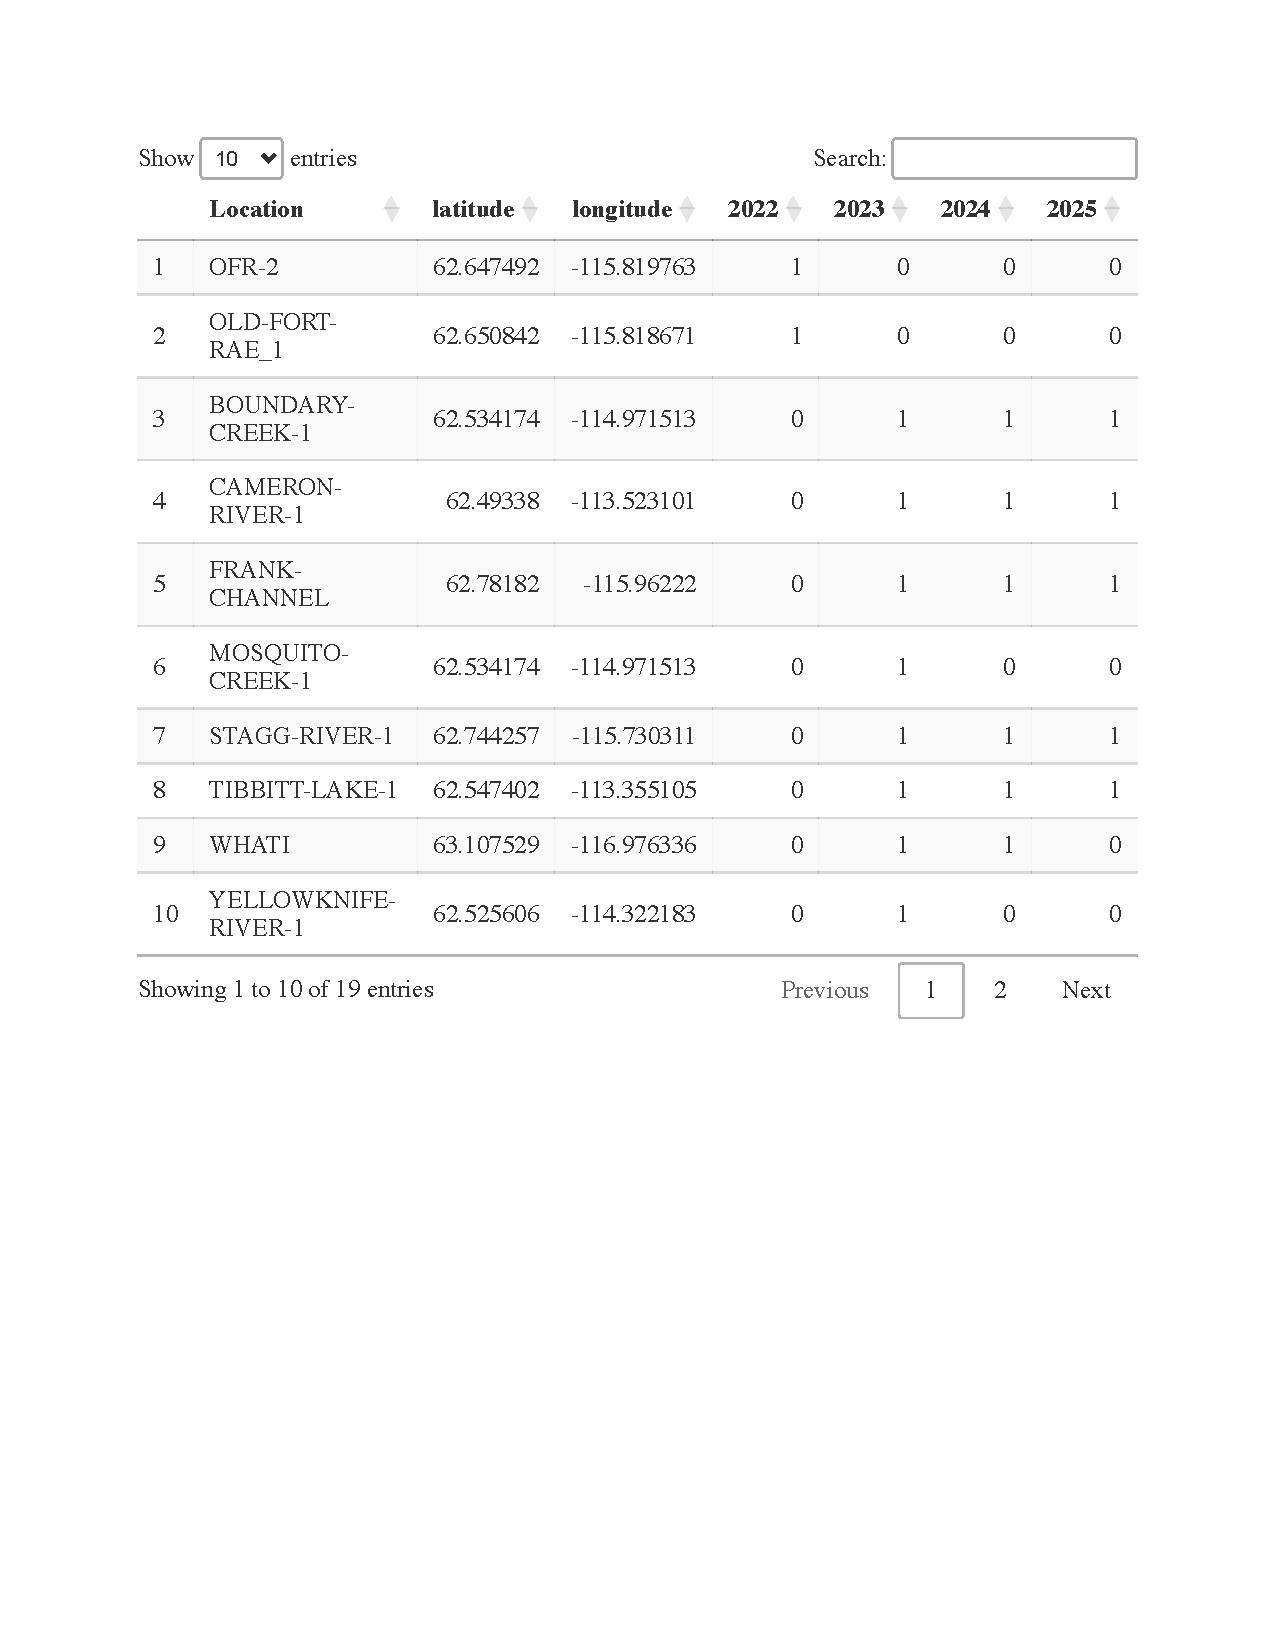
\includegraphics[keepaspectratio]{nsma_files/figure-pdf/tbl-loc-summary-1.pdf}}

}

\end{table}%

\subsection{Data processing}\label{data-processing}

Media were transferred via hard drive to the University of Alberta in
Edmonton, where they are redundantly stored on a server known as Cirrus.
The recordings were standardized to ensure adherence to the naming
convention of \texttt{LOCATION\_DATETIME}, such as
\texttt{PREDULE-LAKE-1\_20230625\_053500.wav}. Recordings were also
directly uploaded to WildTrax for processing and can be downloaded from
the platform's Recording tab, accessible under Manage \textgreater{}
Download list of recordings (see Figure~\ref{fig-download-recs})

\begin{tcolorbox}[enhanced jigsaw, opacitybacktitle=0.6, colframe=quarto-callout-note-color-frame, rightrule=.15mm, coltitle=black, opacityback=0, title=\textcolor{quarto-callout-note-color}{\faInfo}\hspace{0.5em}{Note}, left=2mm, toprule=.15mm, breakable, bottomtitle=1mm, toptitle=1mm, titlerule=0mm, leftrule=.75mm, colback=white, colbacktitle=quarto-callout-note-color!10!white, arc=.35mm, bottomrule=.15mm]

Advanced users can also use \texttt{wildrtrax} with
\texttt{wt\_get\_sync(api\ =\ "organization\_recording\_summary",\ option\ =\ "data",\ organization\ =\ 5425)}.
Ensure you have correct access to the Organization as these projects are
not currently published 2026-03-25.

\end{tcolorbox}

\begin{figure}

\centering{

\pandocbounded{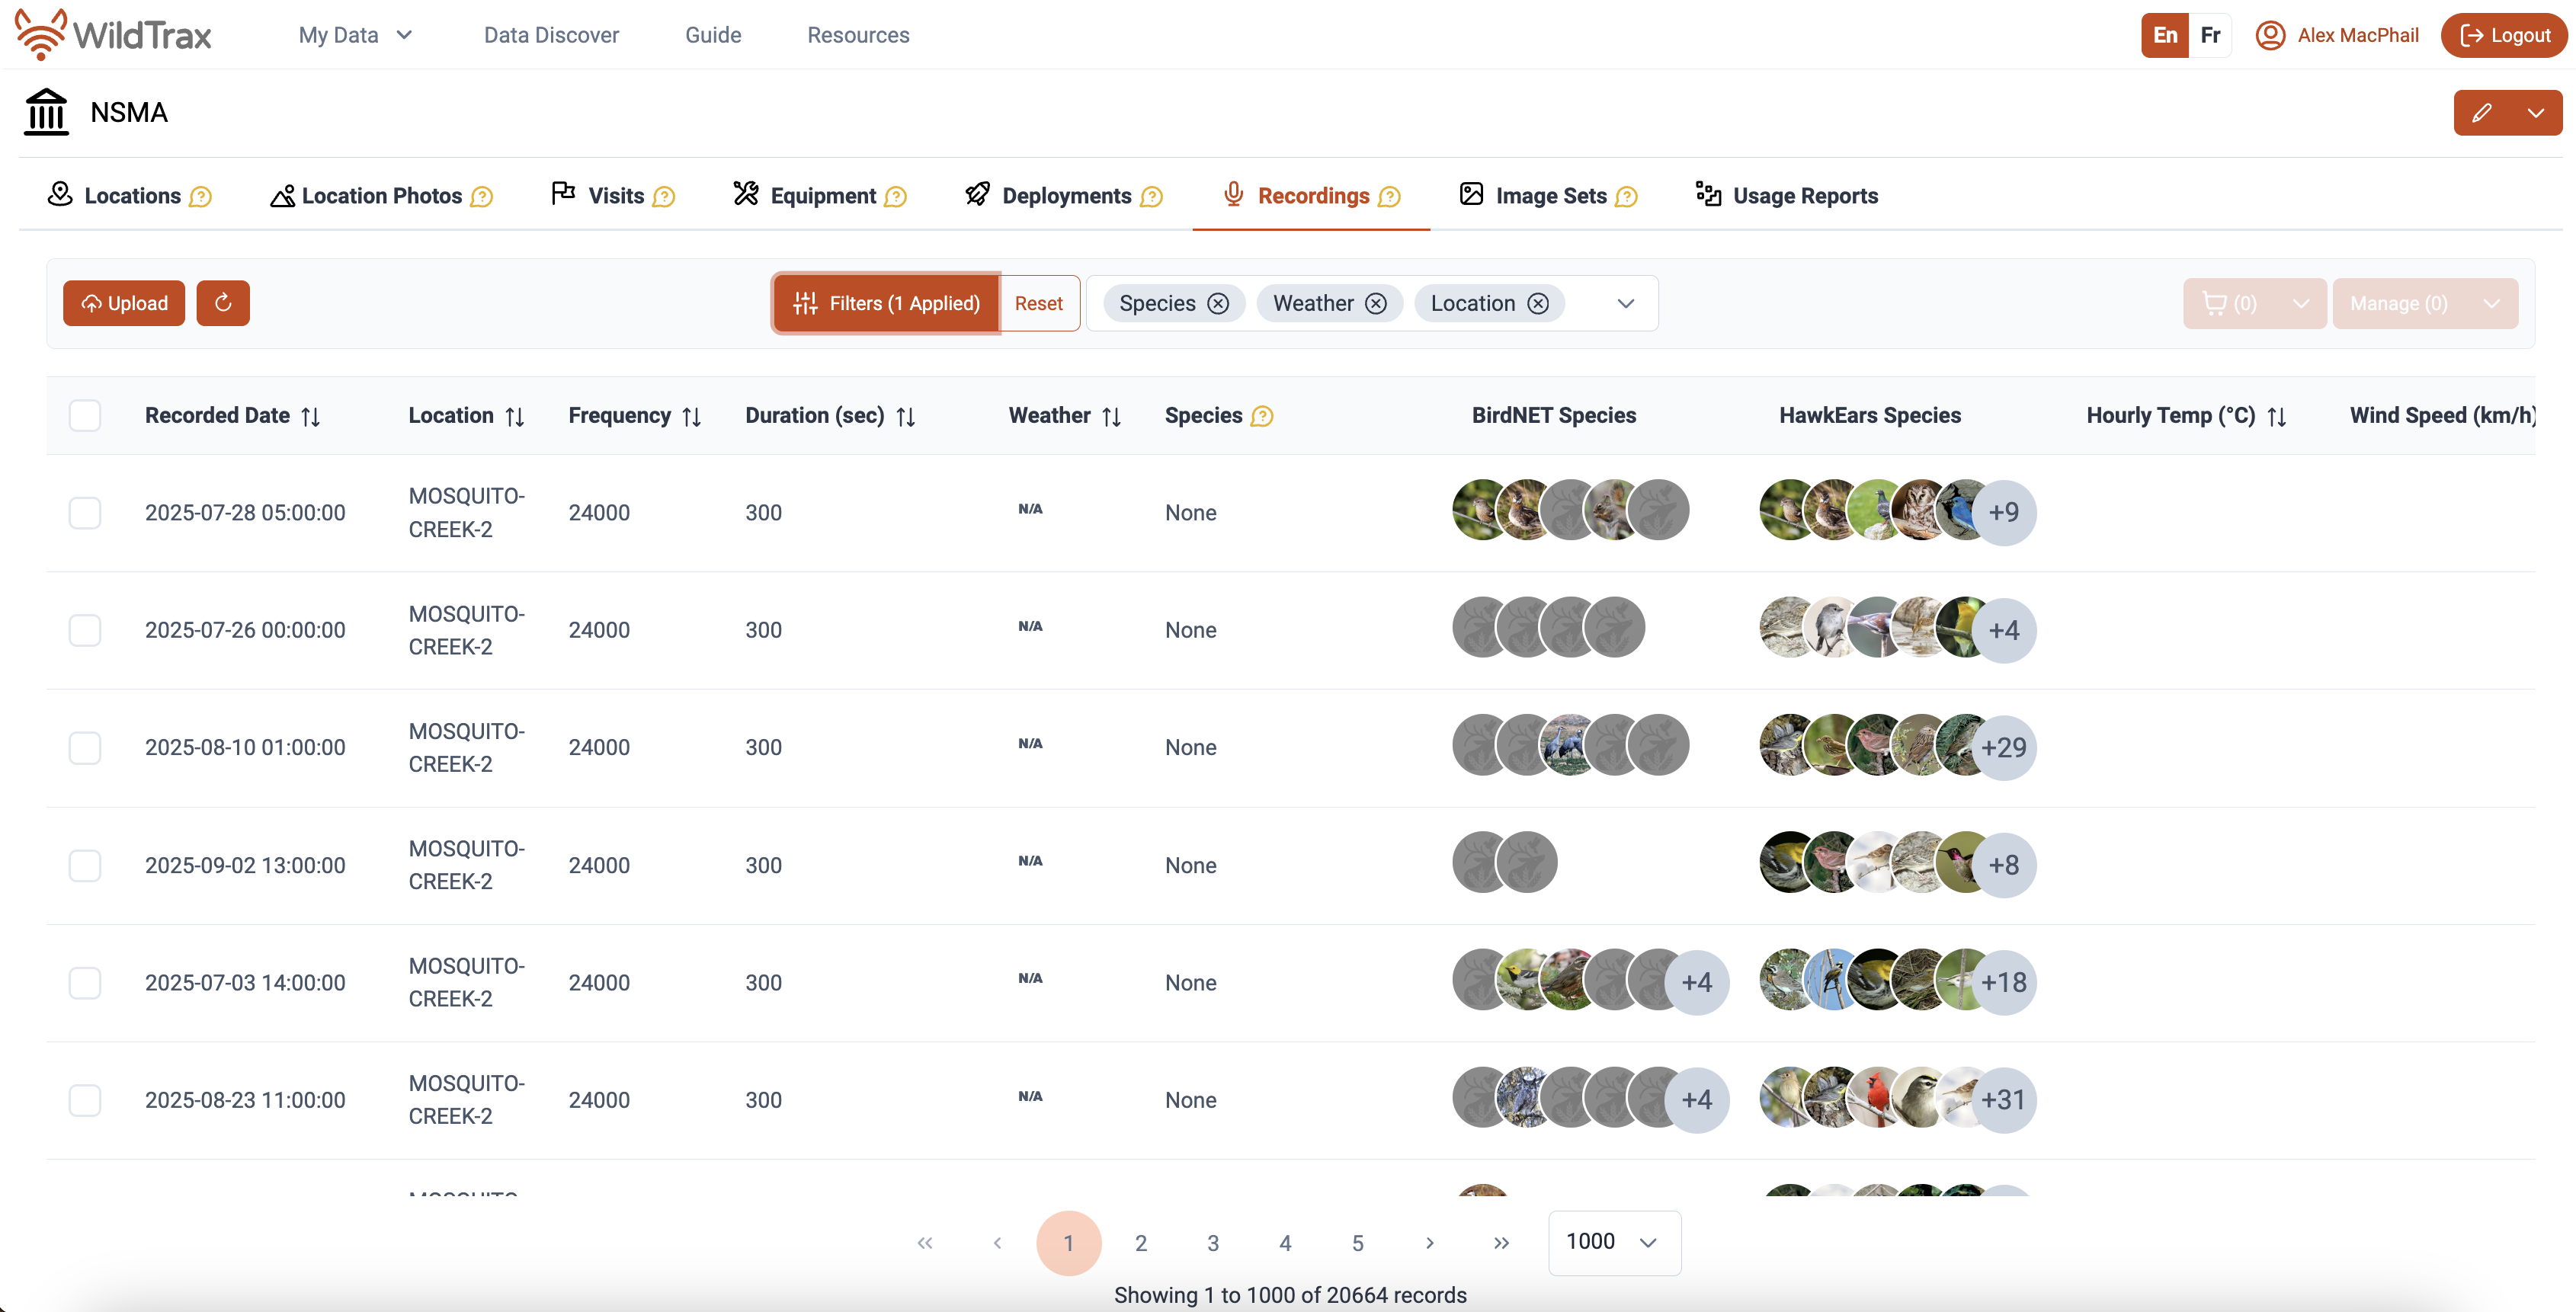
\includegraphics[keepaspectratio]{assets/nsma-recs.png}}

}

\caption{\label{fig-download-recs}Downloading a list of recordings from
WildTrax}

\end{figure}%

The principal goal for data processing was to describe the acoustic
community of species heard at locations while choosing a large enough
subset of recordings for analyses. To ensure balanced replication, for
each location and year surveyed, four randomly selected recordings were
processed for 3-minutes between the hours of 3:00 AM - 7:59 AM (dawn
period) and 20:00 - 23:59 PM (dusk period), ideally on four separate
dates. Four samples ensures that there is minimum number of samples
being able to detect most species. Tags are made using count-removal
(see Farnsworth et al. (2002), Sólymos et al. (2018)) where tags are
only made at the time of first detection of each individual heard on the
recordings. We also verified that all tags that were created were
checked by a second observer (n = 3.38) to ensure accuracy of detections
(see Table~\ref{tbl-verified}). Amphibian abundance was estimated at the
time of first detection using the
\href{https://www.usgs.gov/centers/eesc/science/north-american-amphibian-monitoring-program}{North
American Amphibian Monitoring Program} with abundance of species being
estimated on the scale of ``calling intensity index'' (CI) of 1 - 3.
Mammals such as Red Squirrel, were also noted on the recordings. After
the data are processed in WildTrax, the
\href{https://abbiodiversity.github.io/wildrtrax/}{wildrtrax} package is
used to download the data into a standard format prepared for analysis.
The \texttt{wt\_download\_report} function downloads the data directly
to a R framework for easy manipulation (see
\href{https://abbiodiversity.github.io/wildrtrax/articles/apis.html}{wildrtrax
APIs}).

\begin{figure}

\centering{

\pandocbounded{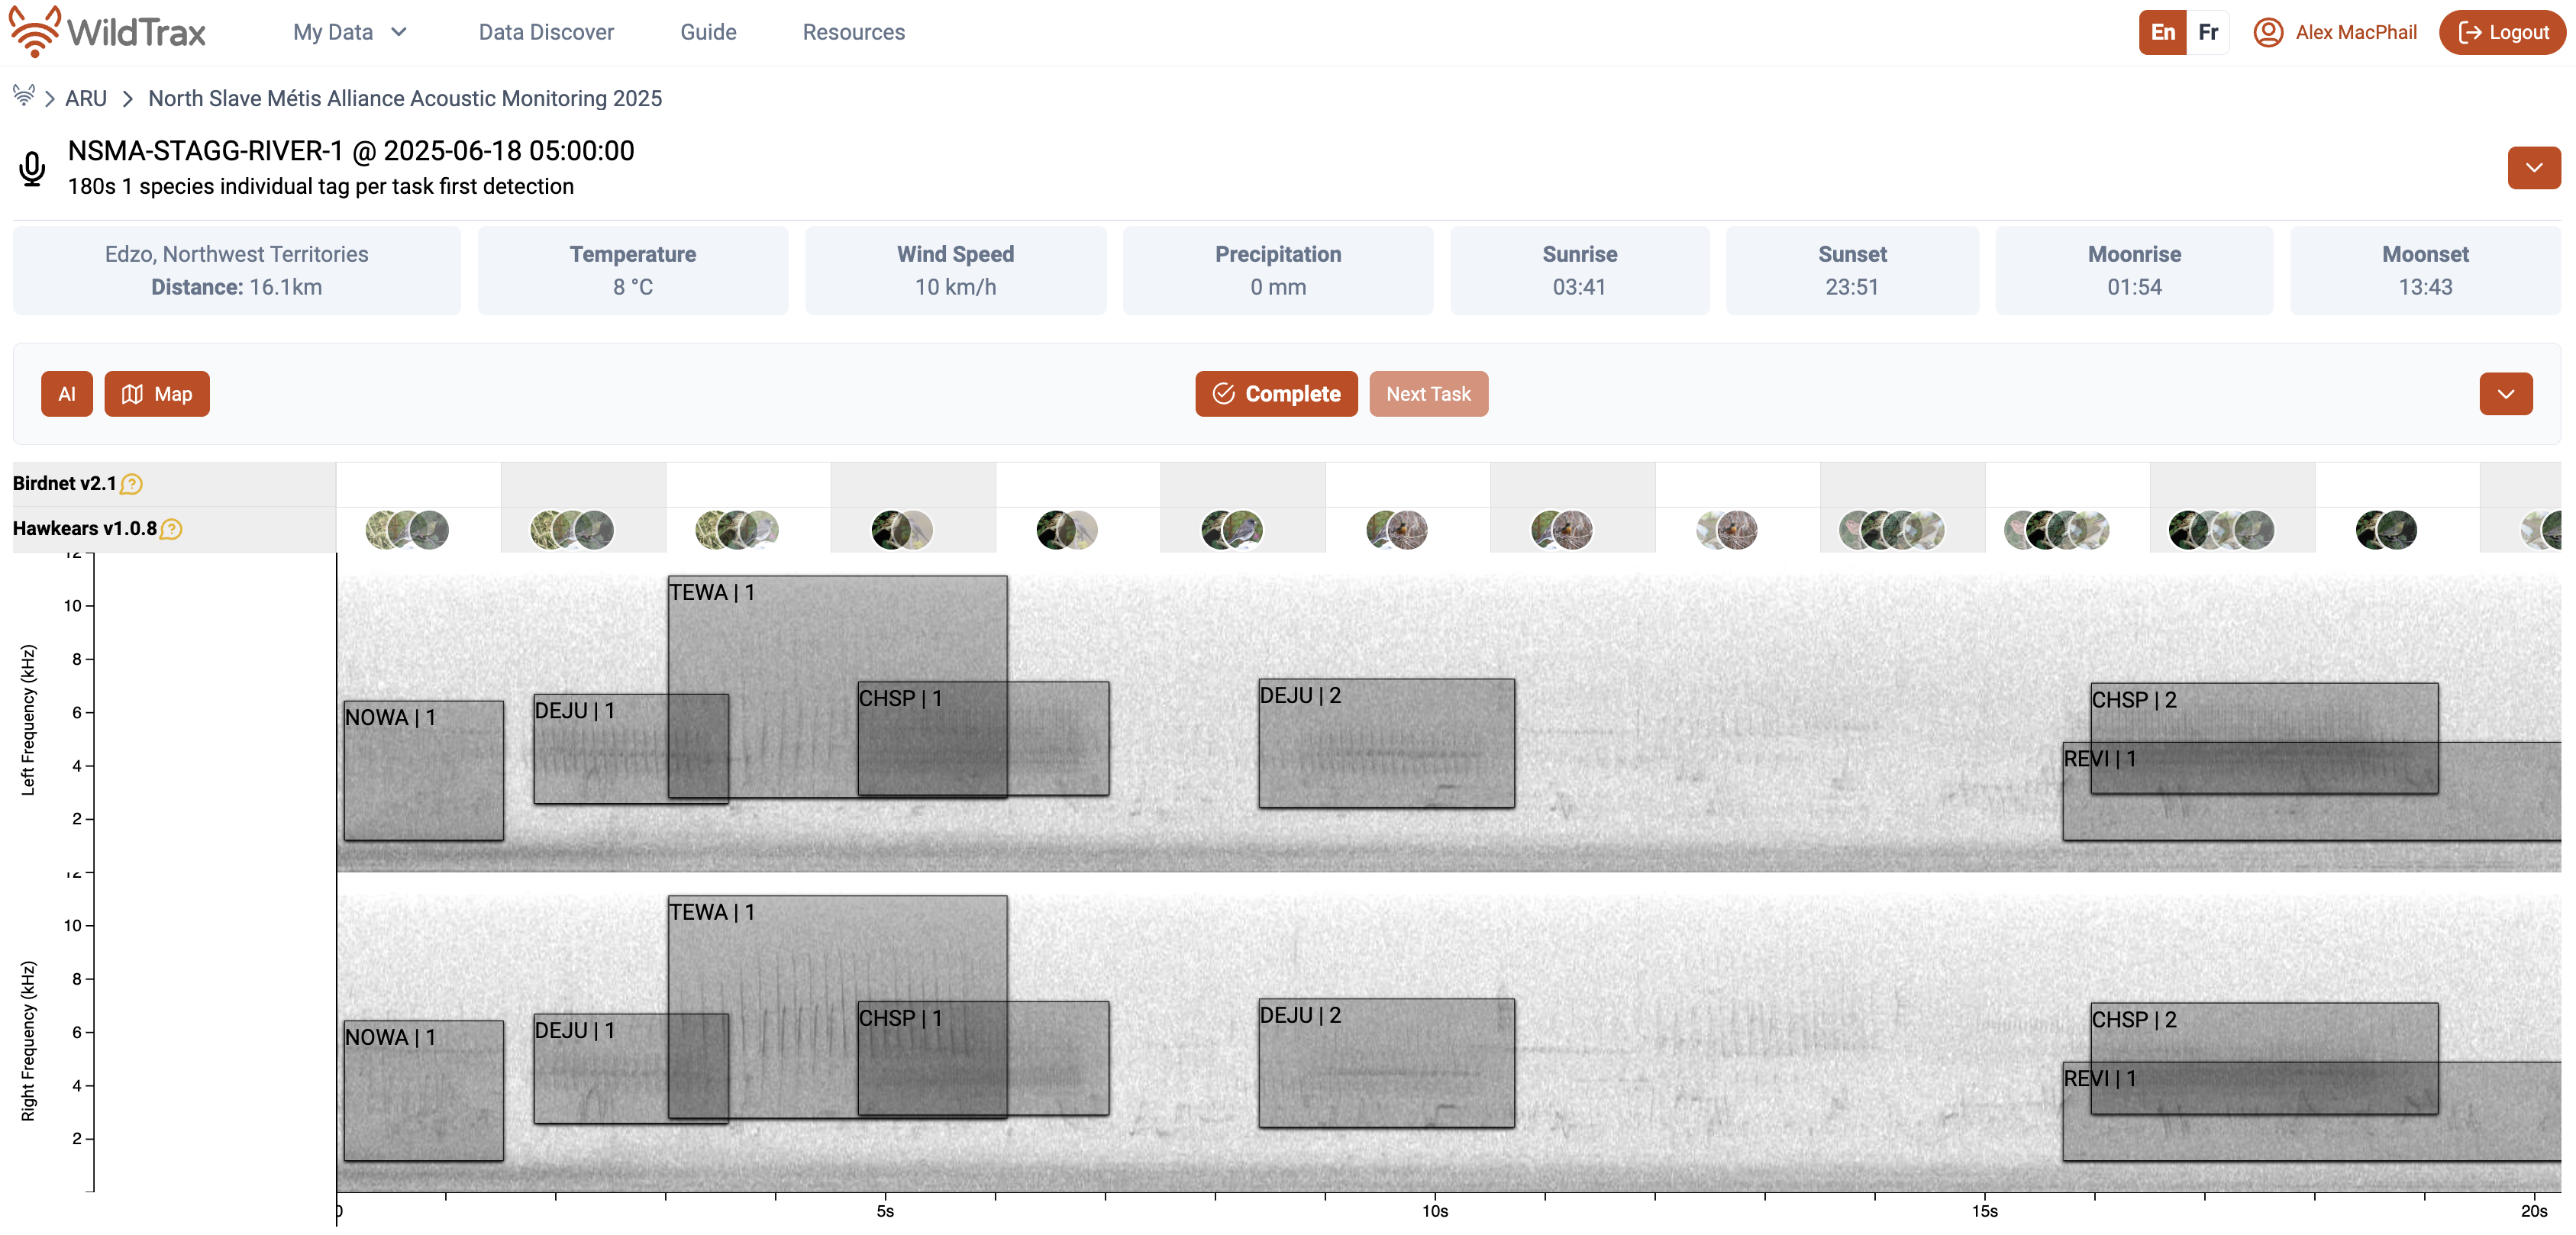
\includegraphics[keepaspectratio]{assets/nsma-acousticprocessing.png}}

}

\caption{\label{fig-acousticprocessing}WildTrax Acoustic Processing
Interface (Version 1)}

\end{figure}%

\begin{longtable}[]{@{}lrr@{}}

\caption{\label{tbl-verified}Proportion of tags verified}

\tabularnewline

\toprule\noalign{}
Tag is verified & Count & Proportion \\
\midrule\noalign{}
\endhead
\bottomrule\noalign{}
\endlastfoot
FALSE & 545 & 32.29 \\
TRUE & 1086 & 64.34 \\
NA & 57 & 3.38 \\

\end{longtable}

\subsection{Analysis}\label{analysis}

To evaluate species richness and activity patterns, we grouped the data
by year and location using the \texttt{dplyr} R package identifying
unique species detected in tasks processed within WildTrax. This enabled
the creation of species richness and activity plots for the results
using \texttt{ggplot}. We used the \texttt{vegan} package in R to
construct a species accumulation curve, assessing the sampling effort
required to capture species richness. The analysis utilized a
species-by-site matrix and employed a randomized accumulation method
with 100 permutations to provide robust estimates of species richness as
sampling sites increased. To support site prioritization, we created a
composite score through a weighted sum of three factors: the need for
repeat surveys, the species richness observed at each site, and any
existing project-specific priorities, here, any species-at-risk.

\section{Results}\label{results}

\begin{figure}

\centering{

\pandocbounded{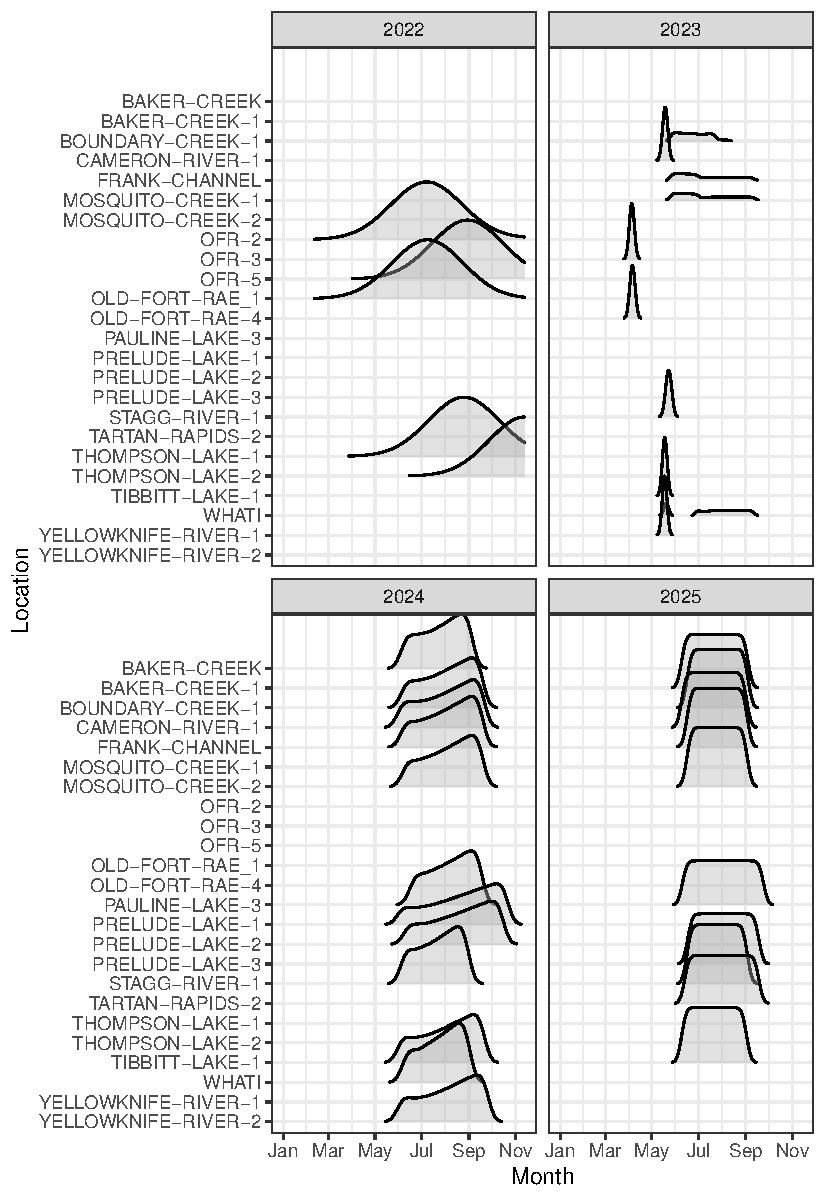
\includegraphics[keepaspectratio]{nsma_files/figure-pdf/fig-all-recs-1.pdf}}

}

\caption{\label{fig-all-recs}All recordings collected from the ARU
monitoring program}

\end{figure}%

A total of 45549 recordings were collected across all three years (see
Figure~\ref{fig-all-recs}). Species richness increased at most locations
sampled in 2024 compared to 2023, likely reflecting differences in
sampling effort (see Figure~\ref{fig-spp-rich-locs}). For example,
BOUNDARY-CREEK-1 recorded an increase from 16 species in 2023 to 26
species in 2024, while STAGG-RIVER-1 increased from 23 to 25 species.
Similarly, TIBBIT-LAKE-1 and WHATI saw notable increases, with species
counts rising from 14 to 19 and 7 to 11, respectively. Locations sampled
exclusively in 2024, such as MOSQUITO-CREEK-2 and PAULINE-LAKE-3,
recorded species counts of 3 and 7, respectively, adding to the overall
species inventory. In contrast, smaller changes were observed at sites
like CAMERON-RIVER-1, where species richness increased from 8 to 10.

\begin{figure}

\centering{

\pandocbounded{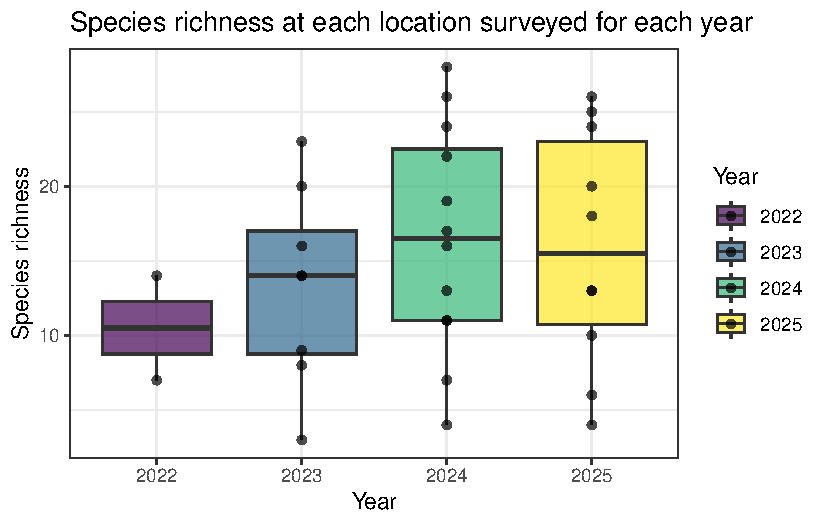
\includegraphics[keepaspectratio]{nsma_files/figure-pdf/fig-spp-rich-locs-1.pdf}}

}

\caption{\label{fig-spp-rich-locs}Species richness at forest monitoring
locations across years}

\end{figure}%

\subsection{Species accumulation}\label{species-accumulation}

The species accumulation curve seen in Figure~\ref{fig-spp-accum}
revealed a steady increase in species richness with additional sampling
sites, reaching a richness of 88 species at the maximum total of
locations surveyed (\emph{n} = 19). Standard deviations declined
consistently with increasing sample size, reflecting greater precision
in richness estimates as sampling effort increased. Richness values
exhibited slightly diminishing returns beyond approximately 15
locations, indicating that additional sampling yielded fewer new species
for the habitats surveyed would plateau suggests that sampling effort at
this time of year was nearly sufficient to capture most vocalizing
species present in the study area.

\begin{figure}

\centering{

\pandocbounded{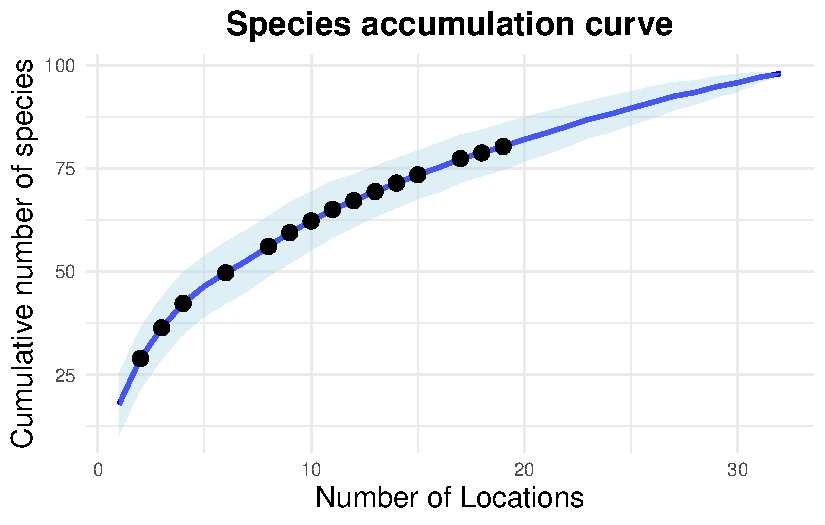
\includegraphics[keepaspectratio]{nsma_files/figure-pdf/fig-spp-accum-1.pdf}}

}

\caption{\label{fig-spp-accum}Species accumulation curve}

\end{figure}%

\subsection{Species through the
season}\label{species-through-the-season}

Figures Figure~\ref{fig-spp-activity-trait} --
Figure~\ref{fig-spp-activity} show seasonal activity patterns by
nesting, trait, migratory strategy, and habitat, respectively. Any
ridgeplots that aren't shown are due to lack of data (i.e.~only one or
two species or guild detections) to plot the data.

\begin{table}

\caption{\label{tbl-bird-guilds}Common bird forest species guilds. For
nesting habitat; Ag = Agricultural, Be = Beach, Bo = Bog, CW =
Coniferous Woodlands, ES = Early Successional, MW = Mixed Woodlands, OW
= Open Woodlands, TSS = Treed/Shrubby Swamp, Ur = Urban. Species from
CW, MW, OW, TSS were used for analysis.}

\centering{

\pandocbounded{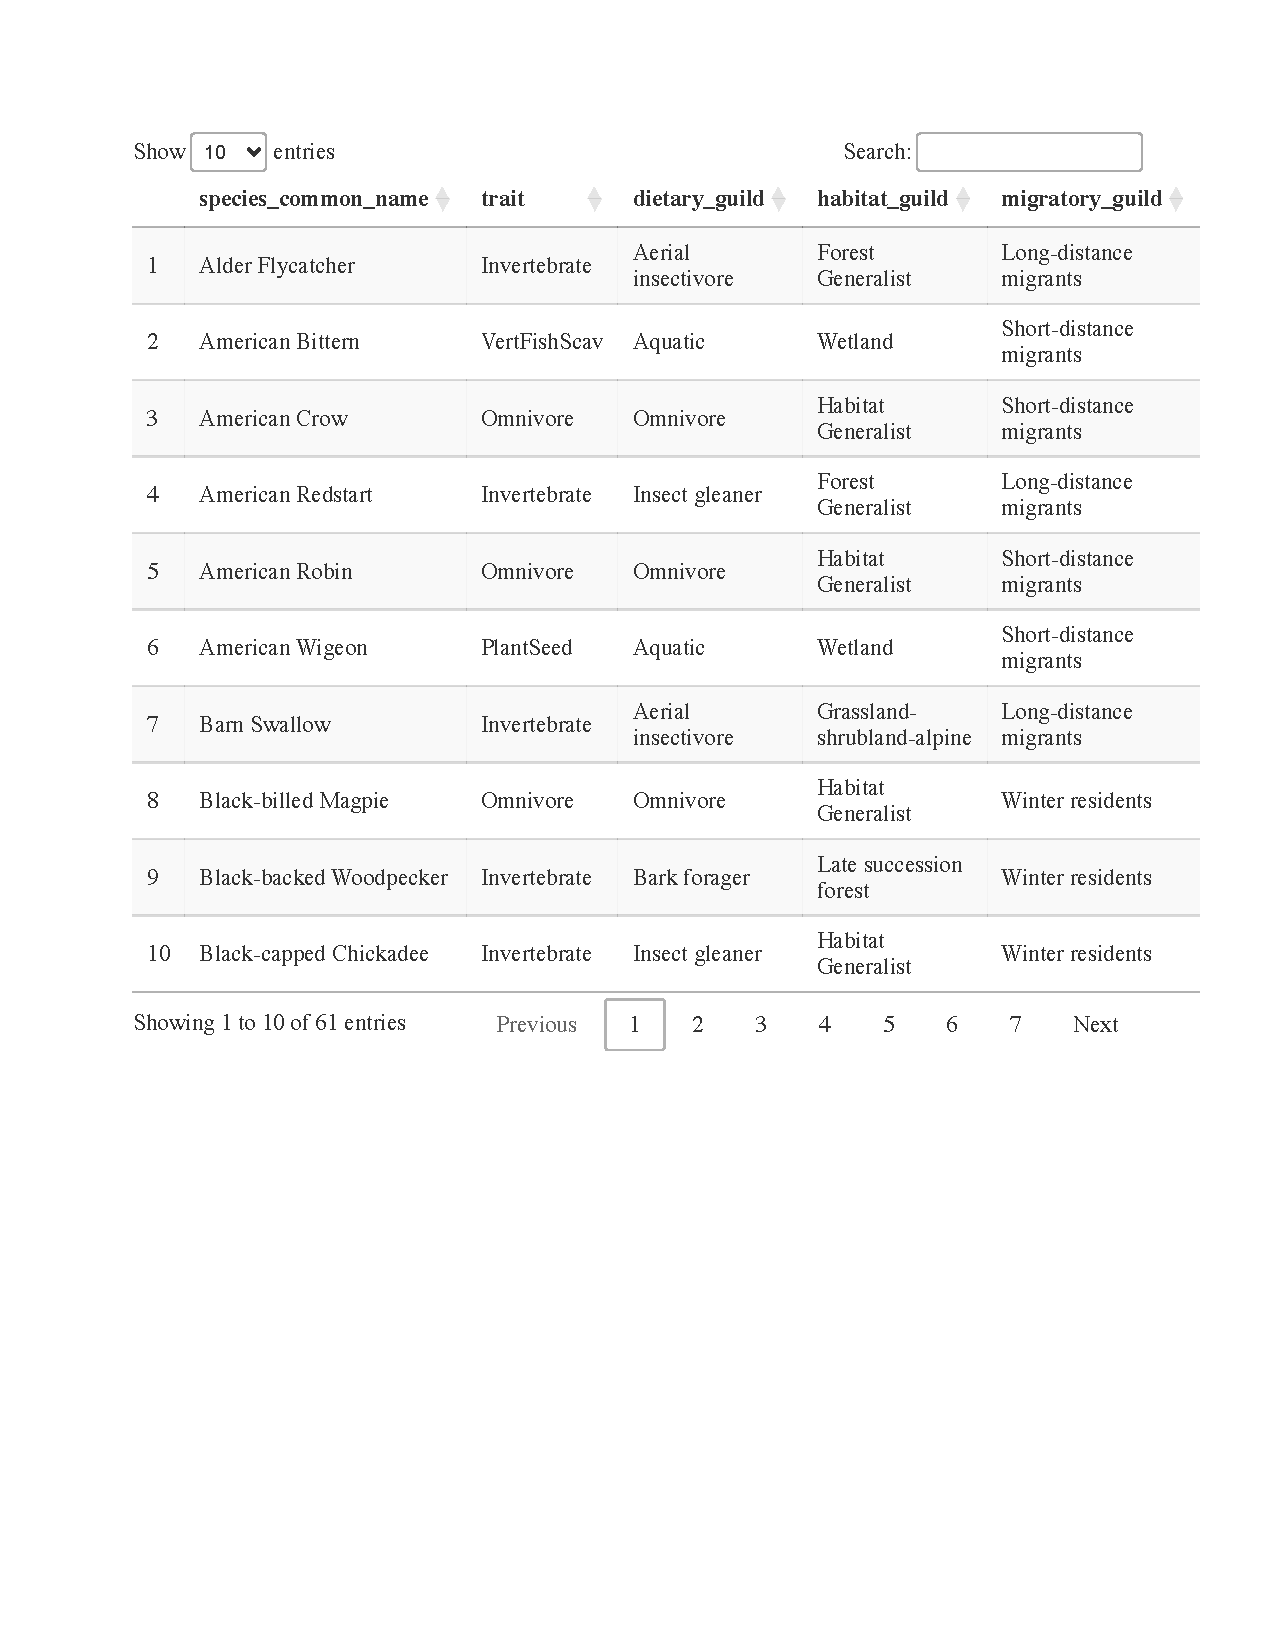
\includegraphics[keepaspectratio]{nsma_files/figure-pdf/tbl-bird-guilds-1.pdf}}

}

\end{table}%

\marginnote{\begin{footnotesize}

\begin{figure}

\centering{

\pandocbounded{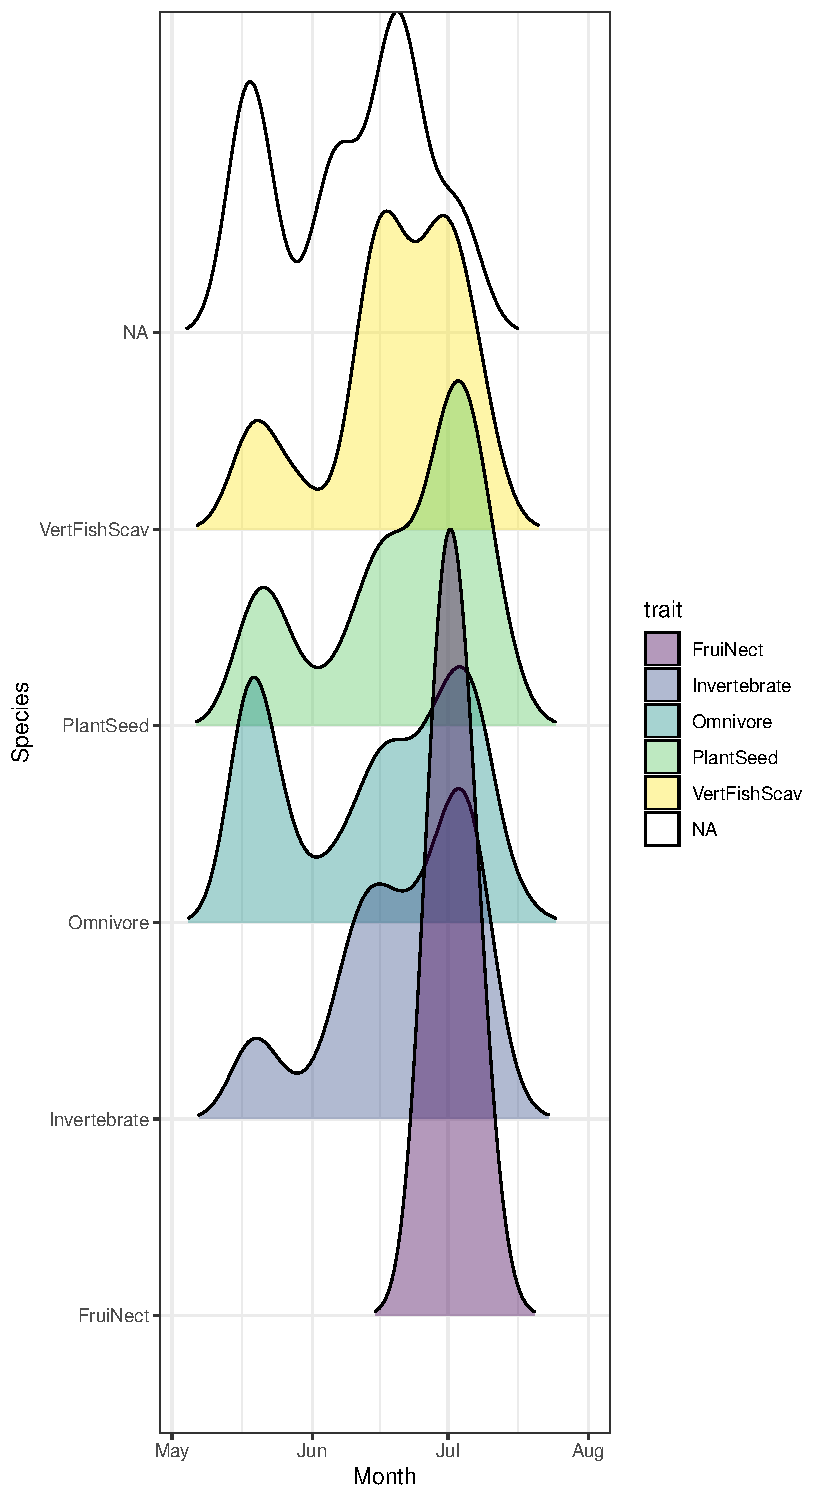
\includegraphics[keepaspectratio]{nsma_files/figure-pdf/fig-spp-activity-trait-1.pdf}}

}

\caption{\label{fig-spp-activity-trait}Species activity}

\end{figure}%

\begin{figure}

\centering{

\pandocbounded{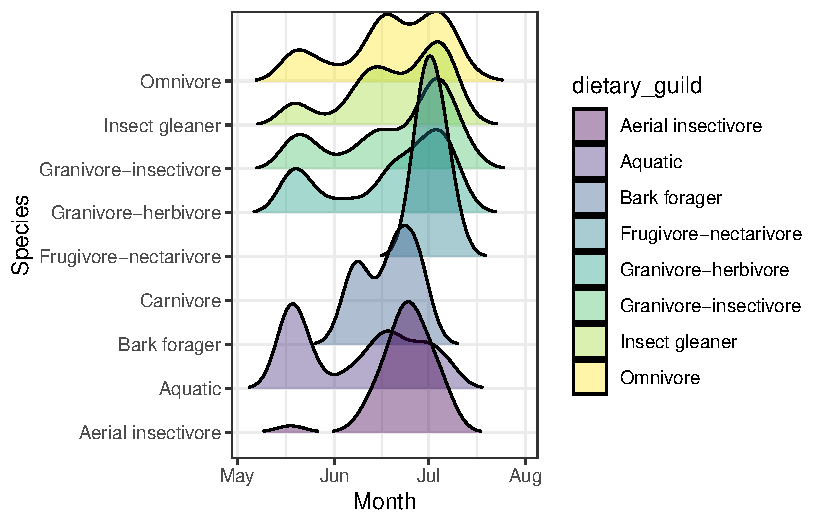
\includegraphics[keepaspectratio]{nsma_files/figure-pdf/fig-spp-activity-dietary-1.pdf}}

}

\caption{\label{fig-spp-activity-dietary}Species activity dietary}

\end{figure}%

{
\makeatletter
\def\LT@makecaption#1#2#3{%
  \noalign{\smash{\hbox{\kern\textwidth\rlap{\kern\marginparsep
  \parbox[t]{\marginparwidth}{%
    \footnotesize{%
      \vspace{(1.1\baselineskip)}
    #1{#2: }\ignorespaces #3}}}}}}%
    }
\makeatother

\begin{figure}

\sidecaption{\label{fig-spp-activity-migratory}Species activity
migratory}

\centering{

\pandocbounded{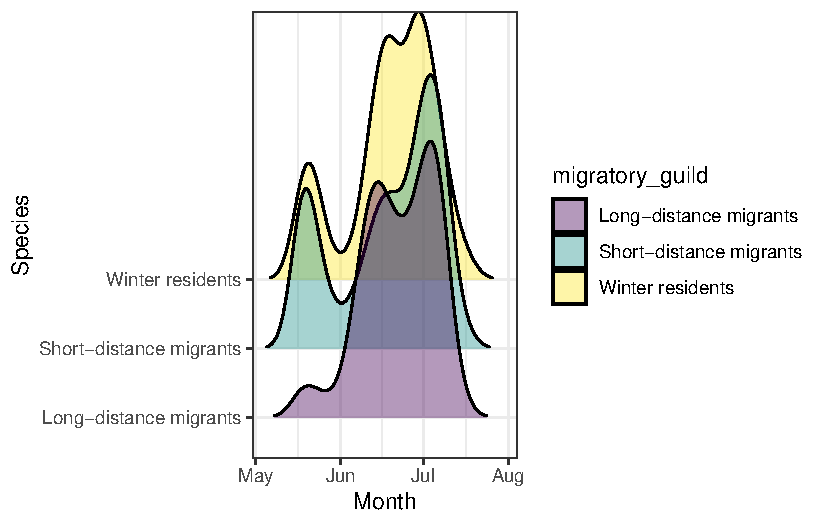
\includegraphics[keepaspectratio]{nsma_files/figure-pdf/fig-spp-activity-migratory-1.pdf}}

}

\end{figure}%

}

\end{footnotesize}}

\begin{figure}

\centering{

\pandocbounded{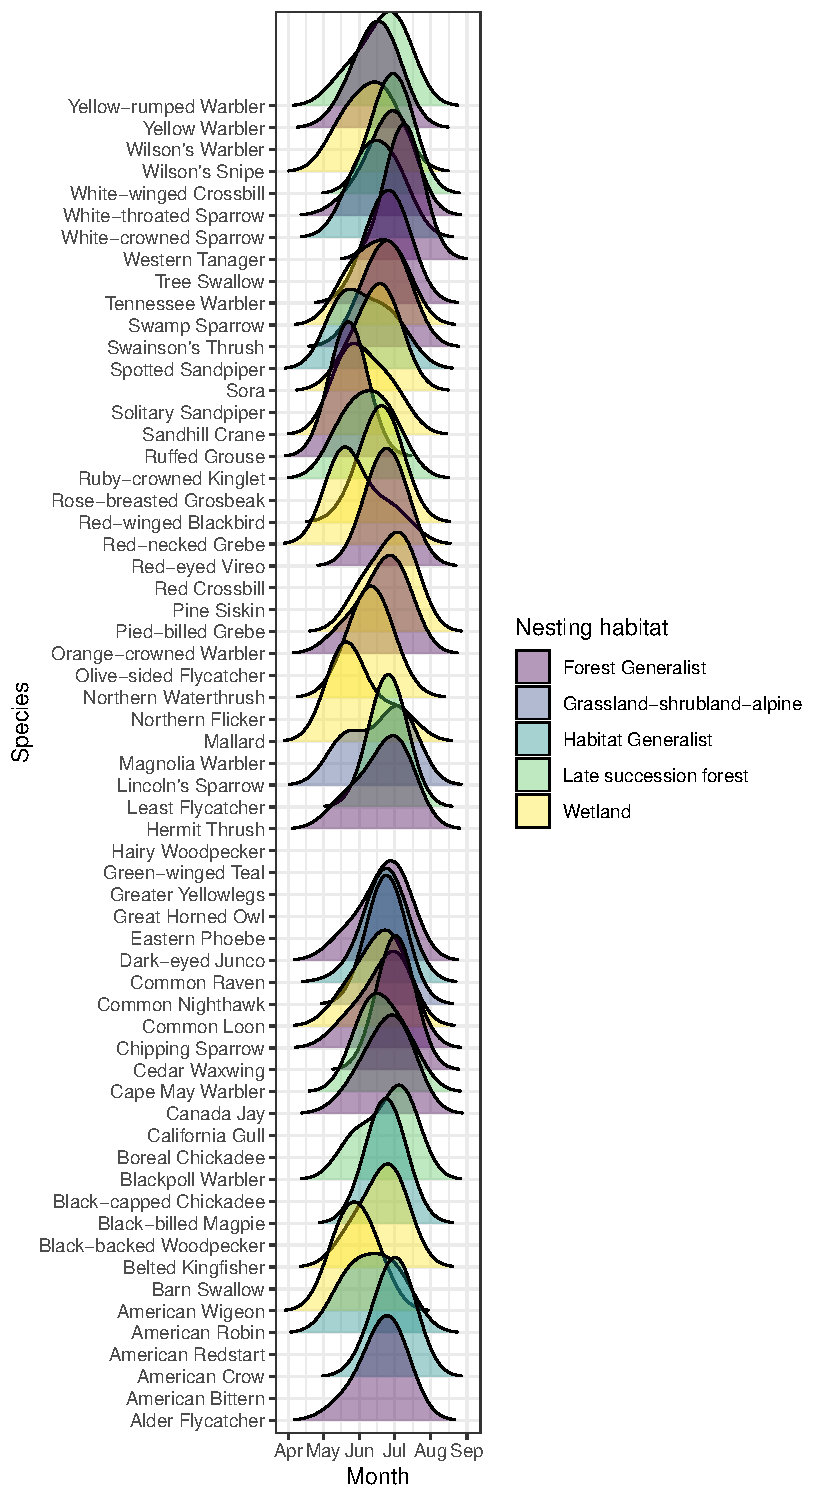
\includegraphics[keepaspectratio]{nsma_files/figure-pdf/fig-spp-activity-1.pdf}}

}

\caption{\label{fig-spp-activity}Species activity}

\end{figure}%

\subsection{Species-at-risk}\label{species-at-risk}

4 species-at-risk were discovered in this data set. Table~\ref{tbl-sar}
outlines the species and which locations they were detected at.
Species-at-risk status was pulled from the
\href{https://www.nature.com/articles/s41597-022-01381-8}{CANSAR
database}.

\begin{table}

\caption{\label{tbl-sar}Species-at-risk detections}

\centering{

\pandocbounded{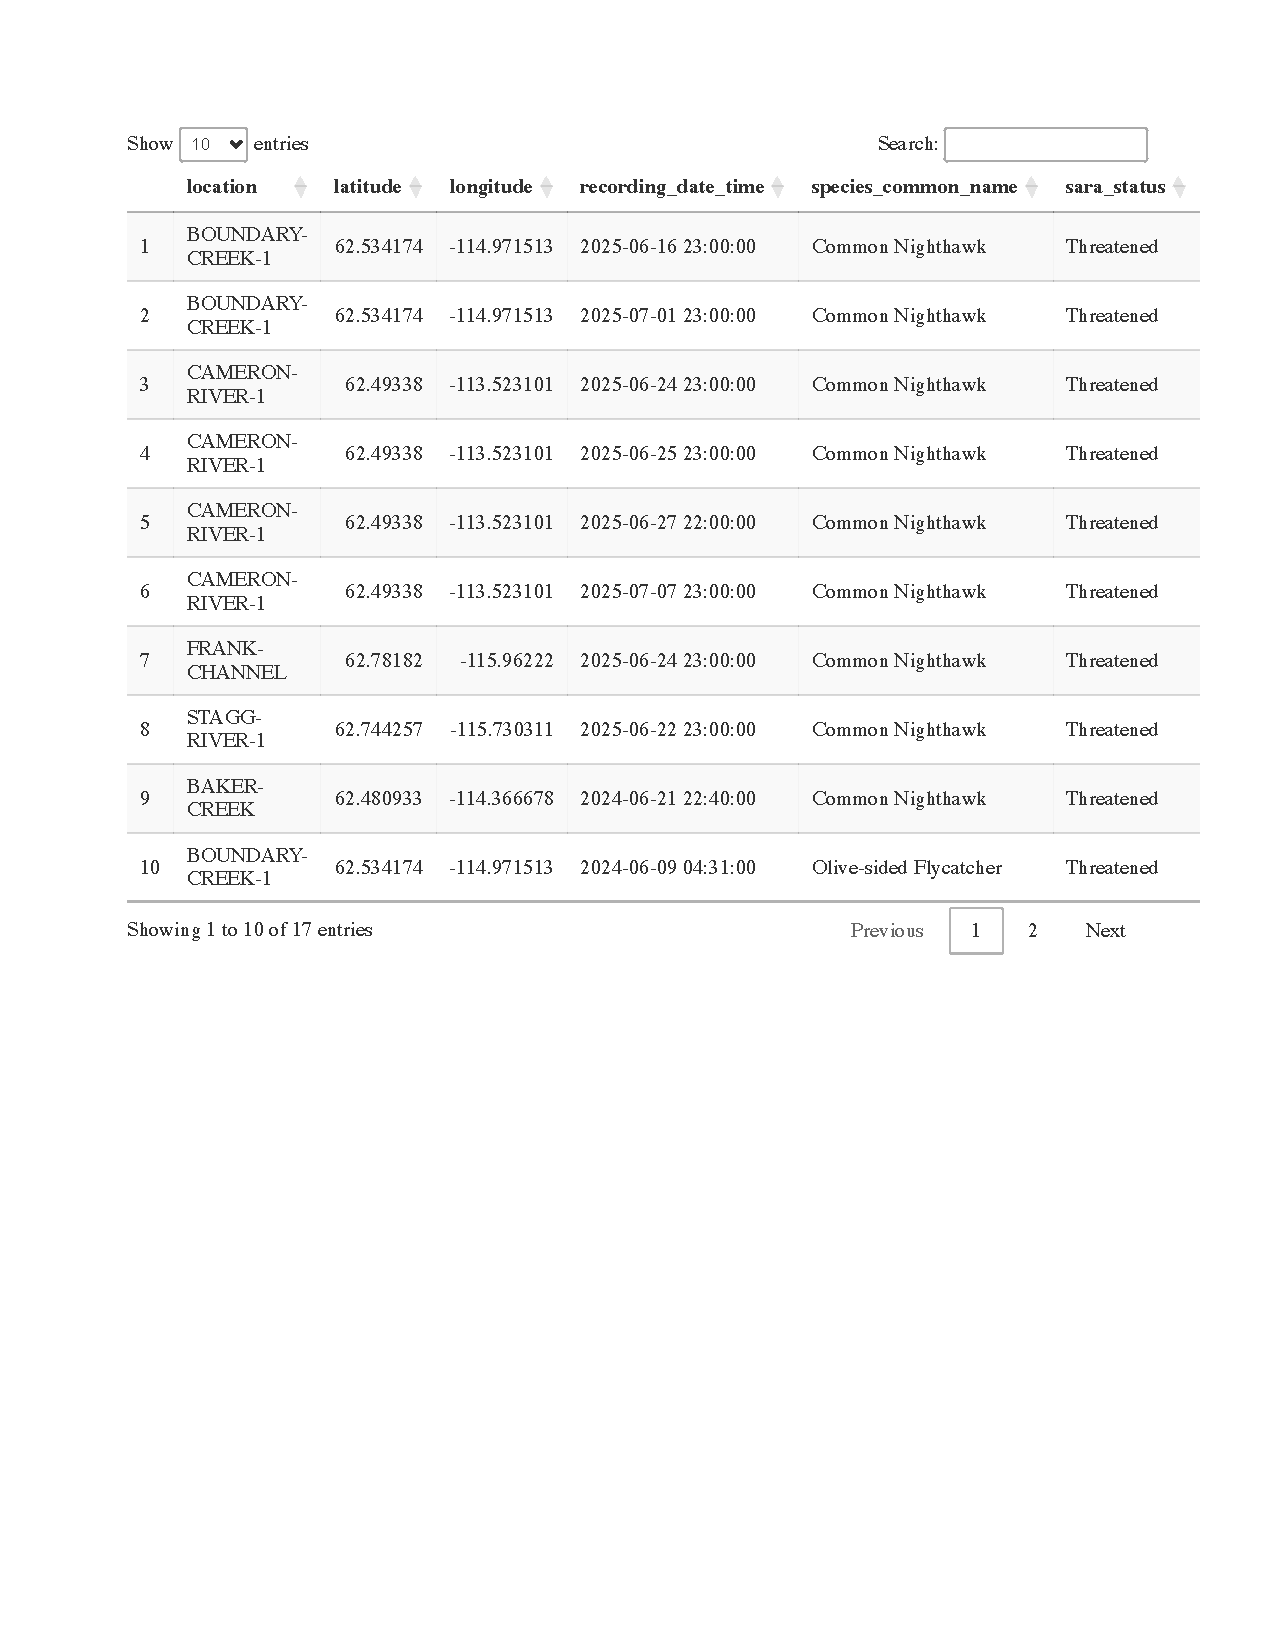
\includegraphics[keepaspectratio]{nsma_files/figure-pdf/tbl-sar-1.pdf}}

}

\end{table}%

\begin{Shaded}
\begin{Highlighting}[]
\NormalTok{soi }\OtherTok{\textless{}{-}} \FunctionTok{c}\NormalTok{(}
  \StringTok{"Bank Swallow"}\NormalTok{,}
  \StringTok{"Barn Swallow"}\NormalTok{,}
  \StringTok{"Common Nighthawk"}\NormalTok{,}
  \StringTok{"Evening Grosbeak"}\NormalTok{,}
  \StringTok{"Harris\textquotesingle{}s Sparrow"}\NormalTok{,}
  \StringTok{"Horned Grebe"}\NormalTok{,}
  \StringTok{"Lesser Yellowlegs"}\NormalTok{,}
  \StringTok{"Olive{-}sided Flycatcher"}\NormalTok{,}
  \StringTok{"Red{-}necked phalarope"}\NormalTok{,}
  \StringTok{"Rusty Blackbird"}\NormalTok{,}
  \StringTok{"Short{-}billed Dowitcher"}\NormalTok{,}
  \StringTok{"Short{-}eared Owl"}\NormalTok{,}
  \StringTok{"Snowy Owl"}\NormalTok{,}
  \StringTok{"Yellow Rail"}
\NormalTok{)}

\NormalTok{nsma\_main }\SpecialCharTok{|\textgreater{}}
  \FunctionTok{filter}\NormalTok{(species\_common\_name }\SpecialCharTok{\%in\%}\NormalTok{ soi) }\SpecialCharTok{|\textgreater{}}
  \FunctionTok{select}\NormalTok{(location, latitude, longitude, recording\_date\_time, species\_common\_name) }
\DocumentationTok{\#\# \# A tibble: 28 x 5}
\DocumentationTok{\#\#    location         latitude longitude recording\_date\_time species\_common\_name}
\DocumentationTok{\#\#    \textless{}chr\textgreater{}               \textless{}dbl\textgreater{}     \textless{}dbl\textgreater{} \textless{}dttm\textgreater{}              \textless{}chr\textgreater{}              }
\DocumentationTok{\#\#  1 BOUNDARY{-}CREEK{-}1     62.5     {-}115. 2025{-}06{-}16 23:00:00 Common Nighthawk   }
\DocumentationTok{\#\#  2 BOUNDARY{-}CREEK{-}1     62.5     {-}115. 2025{-}07{-}01 23:00:00 Common Nighthawk   }
\DocumentationTok{\#\#  3 CAMERON{-}RIVER{-}1      62.5     {-}114. 2025{-}06{-}24 23:00:00 Common Nighthawk   }
\DocumentationTok{\#\#  4 CAMERON{-}RIVER{-}1      62.5     {-}114. 2025{-}06{-}25 23:00:00 Common Nighthawk   }
\DocumentationTok{\#\#  5 CAMERON{-}RIVER{-}1      62.5     {-}114. 2025{-}06{-}25 23:00:00 Common Nighthawk   }
\DocumentationTok{\#\#  6 CAMERON{-}RIVER{-}1      62.5     {-}114. 2025{-}06{-}27 22:00:00 Common Nighthawk   }
\DocumentationTok{\#\#  7 CAMERON{-}RIVER{-}1      62.5     {-}114. 2025{-}07{-}07 23:00:00 Common Nighthawk   }
\DocumentationTok{\#\#  8 FRANK{-}CHANNEL        62.8     {-}116. 2025{-}06{-}24 23:00:00 Common Nighthawk   }
\DocumentationTok{\#\#  9 FRANK{-}CHANNEL        62.8     {-}116. 2025{-}06{-}24 23:00:00 Common Nighthawk   }
\DocumentationTok{\#\# 10 FRANK{-}CHANNEL        62.8     {-}116. 2025{-}06{-}24 23:00:00 Common Nighthawk   }
\DocumentationTok{\#\# \# i 18 more rows}
\end{Highlighting}
\end{Shaded}

\section{Discussion}\label{discussion}

To ensure the integrity and consistency of a long-term monitoring
program, it is important to maintain a consistent survey schedule and
timing each year when deploying ARUs. This consistency helps reduce
variation caused by seasonal differences in species presence or
activity. Additionally, the importance of regular maintenance and
calibration of ARU equipment, particularly microphones, which degrade
over time and can affect data quality if not properly managed after
prolonged field use (see Turgeon, Wilgenburg, and Drake (2017)).
Surveying locations with a history of monitoring over multiple years is
key to tracking changes in species composition and detecting long-term
trends. By including sites with both high and low species diversity, we
can better understand how habitats and species ranges are shifting over
time. Sites where species-at-risk are present are also prioritized to
support conservation efforts. Together, these considerations inform the
prioritized list of key sampling sites across the NSMA region, as
summarized in Table Table~\ref{tbl-prioritization}.

\begin{Shaded}
\begin{Highlighting}[]
\NormalTok{repeat\_priority }\OtherTok{\textless{}{-}}\NormalTok{ locs\_summary }\SpecialCharTok{|\textgreater{}}
  \FunctionTok{rowwise}\NormalTok{() }\SpecialCharTok{|\textgreater{}}
  \FunctionTok{mutate}\NormalTok{(}\AttributeTok{priority =} \FunctionTok{sum}\NormalTok{(}\FunctionTok{c\_across}\NormalTok{(}\StringTok{\textasciigrave{}}\AttributeTok{2022}\StringTok{\textasciigrave{}}\SpecialCharTok{:}\StringTok{\textasciigrave{}}\AttributeTok{2025}\StringTok{\textasciigrave{}}\NormalTok{), }\AttributeTok{na.rm =} \ConstantTok{TRUE}\NormalTok{)) }\SpecialCharTok{|\textgreater{}}
  \FunctionTok{ungroup}\NormalTok{() }\SpecialCharTok{|\textgreater{}}
  \FunctionTok{arrange}\NormalTok{(}\SpecialCharTok{{-}}\NormalTok{priority)}

\NormalTok{rich\_priority }\OtherTok{\textless{}{-}}\NormalTok{ spp\_rich\_location }\SpecialCharTok{|\textgreater{}} \FunctionTok{group\_by}\NormalTok{(location) }\SpecialCharTok{|\textgreater{}} \FunctionTok{summarise}\NormalTok{(}\AttributeTok{priority =} \FunctionTok{mean}\NormalTok{(species\_count)) }\SpecialCharTok{|\textgreater{}} \FunctionTok{arrange}\NormalTok{(}\SpecialCharTok{{-}}\NormalTok{priority)}

\NormalTok{soi\_priority }\OtherTok{\textless{}{-}}\NormalTok{ nsma\_main }\SpecialCharTok{|\textgreater{}}
  \FunctionTok{filter}\NormalTok{(species\_common\_name }\SpecialCharTok{\%in\%}\NormalTok{ soi) }\SpecialCharTok{|\textgreater{}}
  \FunctionTok{select}\NormalTok{(location, latitude, longitude, recording\_date\_time, species\_common\_name)  }\SpecialCharTok{|\textgreater{}}
  \FunctionTok{group\_by}\NormalTok{(location) }\SpecialCharTok{|\textgreater{}}
  \FunctionTok{summarise}\NormalTok{(}\AttributeTok{priority =} \FunctionTok{n\_distinct}\NormalTok{(species\_common\_name))}

\NormalTok{prioritization\_matrix }\OtherTok{\textless{}{-}}\NormalTok{ repeat\_priority }\SpecialCharTok{|\textgreater{}}
  \FunctionTok{rename}\NormalTok{(}\AttributeTok{location =}\NormalTok{ Location) }\SpecialCharTok{|\textgreater{}}
  \FunctionTok{left\_join}\NormalTok{(rich\_priority, }\AttributeTok{by =} \StringTok{"location"}\NormalTok{, }\AttributeTok{suffix =} \FunctionTok{c}\NormalTok{(}\StringTok{"\_repeat"}\NormalTok{, }\StringTok{"\_rich"}\NormalTok{)) }\SpecialCharTok{|\textgreater{}}
  \FunctionTok{left\_join}\NormalTok{(soi\_priority, }\AttributeTok{by =} \StringTok{"location"}\NormalTok{, }\AttributeTok{suffix =} \FunctionTok{c}\NormalTok{(}\StringTok{""}\NormalTok{, }\StringTok{"\_soi"}\NormalTok{)) }\SpecialCharTok{|\textgreater{}}
  \FunctionTok{mutate}\NormalTok{(}
    \AttributeTok{priority\_repeat =} \FunctionTok{ifelse}\NormalTok{(}\FunctionTok{is.na}\NormalTok{(priority\_repeat), }\DecValTok{0}\NormalTok{, priority\_repeat),}
    \AttributeTok{priority\_rich =} \FunctionTok{ifelse}\NormalTok{(}\FunctionTok{is.na}\NormalTok{(priority\_rich), }\DecValTok{0}\NormalTok{, priority\_rich),}
    \AttributeTok{priority =} \FunctionTok{ifelse}\NormalTok{(}\FunctionTok{is.na}\NormalTok{(priority), }\DecValTok{0}\NormalTok{, priority)}
\NormalTok{  ) }\SpecialCharTok{|\textgreater{}}
  \FunctionTok{mutate}\NormalTok{(}\AttributeTok{combined\_priority =} \FunctionTok{round}\NormalTok{((priority\_repeat }\SpecialCharTok{*} \DecValTok{2} \SpecialCharTok{+}\NormalTok{ priority\_rich }\SpecialCharTok{+}\NormalTok{ priority),}\DecValTok{2}\NormalTok{)) }\SpecialCharTok{|\textgreater{}} \CommentTok{\# Created a weighted{-}sum}
  \FunctionTok{select}\NormalTok{(location, combined\_priority) }\SpecialCharTok{|\textgreater{}}
  \FunctionTok{arrange}\NormalTok{(}\SpecialCharTok{{-}}\NormalTok{combined\_priority)}

\FunctionTok{datatable}\NormalTok{(prioritization\_matrix, }
          \AttributeTok{options =} \FunctionTok{list}\NormalTok{(}
            \AttributeTok{searching =} \ConstantTok{TRUE}\NormalTok{,  }
            \AttributeTok{paging =} \ConstantTok{TRUE}\NormalTok{,    }
            \AttributeTok{pageLength =} \DecValTok{10}   
\NormalTok{          ))}
\end{Highlighting}
\end{Shaded}

\begin{table}

\caption{\label{tbl-prioritization}Prioritization}

\centering{

\pandocbounded{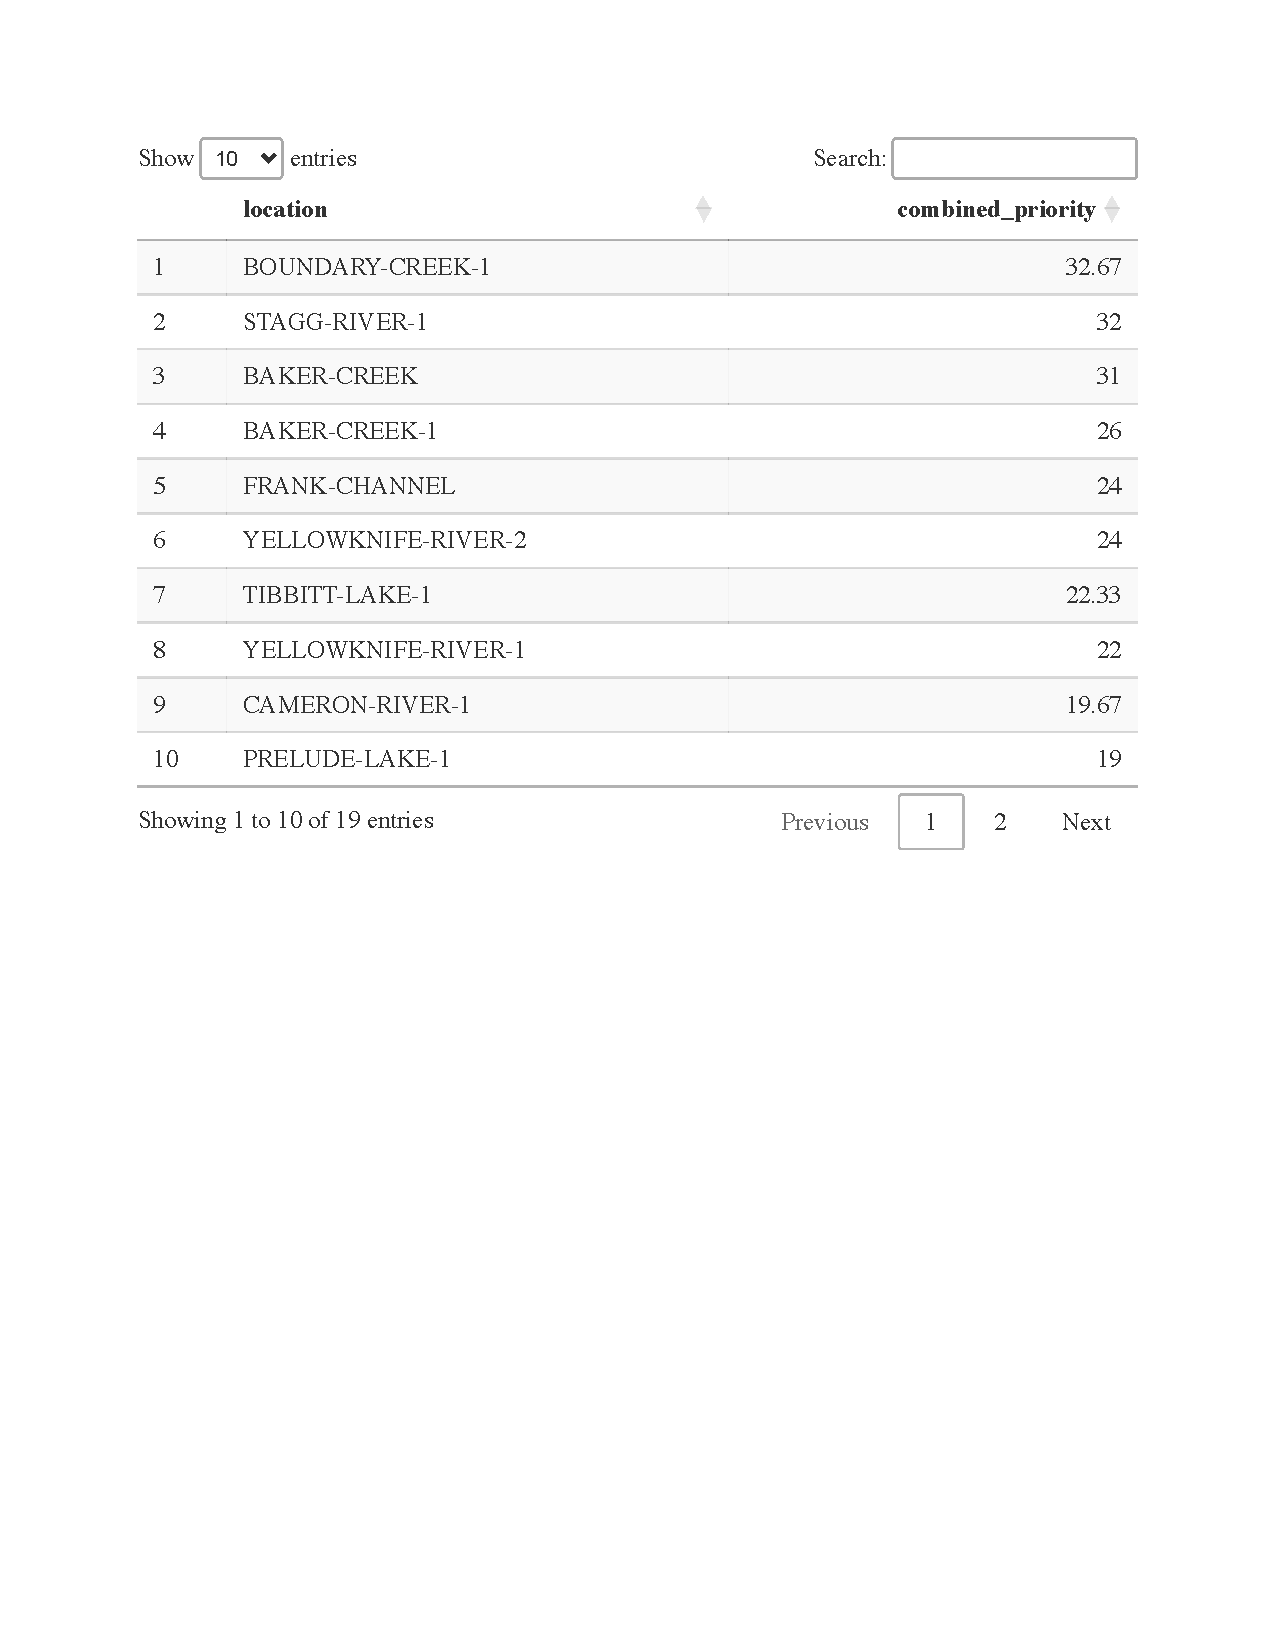
\includegraphics[keepaspectratio]{nsma_files/figure-pdf/tbl-prioritization-1.pdf}}

}

\end{table}%

As this monitoring is led by Indigenous communities, it is guided by
local knowledge, values, and priorities to protect the land and
wildlife. By combining new technologies and sampling technique with
traditional knowledge, the program contributes to building a
comprehensive, long-term understanding of biodiversity in the region.
Ongoing monitoring will help track the impacts of climate change. This
information will help to support communities in protecting their
environment and cultural connections while strengthening resilience for
the future.

\phantomsection\label{refs}
\begin{CSLReferences}{1}{0}
\bibitem[\citeproctext]{ref-abrahms2023climate}
Abrahms, Briana, Neil H Carter, TJ Clark-Wolf, Kaitlyn M Gaynor, Erik
Johansson, Alex McInturff, Anna C Nisi, Kasim Rafiq, and Leigh West.
2023. {``Climate Change as a Global Amplifier of Human--Wildlife
Conflict.''} \emph{Nature Climate Change} 13 (3): 224--34.

\bibitem[\citeproctext]{ref-ackleh2010measuring}
Ackleh, Azmy S, Jacoby Carter, Lauren Cole, Tom Nguyen, Jay Monte, and
Claire Pettit. 2010. {``Measuring and Modeling the Seasonal Changes of
an Urban Green Treefrog (Hyla Cinerea) Population.''} \emph{Ecological
Modelling} 221 (2): 281--89.

\bibitem[\citeproctext]{ref-allan2017recent}
Allan, James R, Oscar Venter, Sean Maxwell, Bastian Bertzky, Kendall
Jones, Yichuan Shi, and James EM Watson. 2017. {``Recent Increases in
Human Pressure and Forest Loss Threaten Many Natural World Heritage
Sites.''} \emph{Biological Conservation} 206: 47--55.

\bibitem[\citeproctext]{ref-vis-scan-amphs}
Cameron, J., A. Crosby, C. Paszkowski, and E. Bayne. 2020. {``Visual
Spectrogram Scanning Paired with an Observation--Confirmation Occupancy
Model Improves the Efficiency and Accuracy of Bioacoustic Anuran
Data.''} \emph{Canadian Journal of Zoology} 98 (11): 733--42.
\url{https://doi.org/10.1139/cjz-2020-0103}.

\bibitem[\citeproctext]{ref-devarajan2020multi}
Devarajan, Kadambari, Toni Lyn Morelli, and Simone Tenan. 2020.
{``Multi-Species Occupancy Models: Review, Roadmap, and
Recommendations.''} \emph{Ecography} 43 (11): 1612--24.

\bibitem[\citeproctext]{ref-fahrig2003effects}
Fahrig, Lenore. 2003. {``Effects of Habitat Fragmentation on
Biodiversity.''} \emph{Annual Review of Ecology, Evolution, and
Systematics} 34 (1): 487--515.

\bibitem[\citeproctext]{ref-farnsworth2002removal}
Farnsworth, George L, Kenneth H Pollock, James D Nichols, Theodore R
Simons, James E Hines, and John R Sauer. 2002. {``A Removal Model for
Estimating Detection Probabilities from Point-Count Surveys.''}
\emph{The Auk} 119 (2): 414--25.

\bibitem[\citeproctext]{ref-gahbauer2022projected}
Gahbauer, Marcel A, Scott R Parker, Joanna X Wu, Cavan Harpur, Brooke L
Bateman, Darroch M Whitaker, Douglas P Tate, Lotem Taylor, and Denis
Lepage. 2022. {``Projected Changes in Bird Assemblages Due to Climate
Change in a Canadian System of Protected Areas.''} \emph{Plos One} 17
(1): e0262116.

\bibitem[\citeproctext]{ref-aru-vs-cams-wolves}
Garland, Laura, Andrew Crosby, Richard Hedley, Stan Boutin, and Erin
Bayne. 2020. {``Acoustic Vs. Photographic Monitoring of Gray Wolves
({Canis lupus}): A Methodological Comparison of Two Passive Monitoring
Techniques.''} \emph{Canadian Journal of Zoology} 98 (3): 219--28.
\url{https://doi.org/10.1139/cjz-2019-0081}.

\bibitem[\citeproctext]{ref-handel2004alaska}
Handel, C. M., and M. N. Cady. 2004. {``Alaska Landbird Monitoring
Survey: Protocol for Setting up and Conducting Point Count Surveys.''}
Technical Report 2004-3. Alaska Science Center: U.S. Geological Survey.

\bibitem[\citeproctext]{ref-hanski2011habitat}
Hanski, Ilkka. 2011. {``Habitat Loss, the Dynamics of Biodiversity, and
a Perspective on Conservation.''} \emph{Ambio} 40 (3): 248--55.

\bibitem[\citeproctext]{ref-knaggs2020avian}
Knaggs, Michelle, Samuel Haché, Scott E Nielsen, Rhiannon F Pankratz,
and Erin Bayne. 2020. {``Avian Response to Wildfire Severity in a
Northern Boreal Region.''} \emph{Forests} 11 (12): 1330.

\bibitem[\citeproctext]{ref-knight2019classification}
Knight, Elly C, and Erin M Bayne. 2019. {``Classification Threshold and
Training Data Affect the Quality and Utility of Focal Species Data
Processed with Automated Audio-Recognition Software.''}
\emph{Bioacoustics} 28 (6): 539--54.

\bibitem[\citeproctext]{ref-lemieux2011state}
Lemieux, Christopher J, Thomas J Beechey, Daniel J Scott, and Paul A
Gray. 2011. {``The State of Climate Change Adaptation in Canada's
Protected Areas Sector.''} \emph{The Canadian Geographer/Le G{é}ographe
Canadien} 55 (3): 301--17.

\bibitem[\citeproctext]{ref-Loeb_2015}
Loeb, Susan C., Thomas J. Rodhouse, Laura E. Ellison, Cori L. Lausen,
Jonathan D. Reichard, Kathryn M. Irvine, Thomas E. Ingersoll, et al.
2015. \emph{A Plan for the North American Bat Monitoring Program
(NABat)}. U.S. Department of Agriculture, Forest Service, Southern
Research Station. \url{https://doi.org/10.2737/srs-gtr-208}.

\bibitem[\citeproctext]{ref-Loeb2015}
Loeb, Susan C., Thomas J. Rodhouse, Lee E. Ellison, et al. 2015. \emph{A
Plan for the North American Bat Monitoring Program (NABat)}. Asheville,
NC: U.S. Department of Agriculture, Forest Service, Southern Research
Station. \url{https://doi.org/10.1898/NWN21-10}.

\bibitem[\citeproctext]{ref-lovett2013peepers}
Lovett, Gary M. 2013. {``When Do Peepers Peep? Climate and the Date of
First Calling in the Spring Peeper (Pseudacris Crucifer) in Southeastern
New York State.''} \emph{Northeastern Naturalist} 20 (2): 333--40.

\bibitem[\citeproctext]{ref-occu-fit}
MacKenzie, Darryl I., and Larissa L. Bailey. 2004. {``Assessing the Fit
of Site-Occupancy Models.''} \emph{Journal of Agricultural, Biological,
and Environmental Statistics} 9 (3): 300--318.
\url{http://www.jstor.org/stable/1400484}.

\bibitem[\citeproctext]{ref-imperfect-occu}
MacKenzie, Darryl I., James D. Nichols, James E. Hines, Melinda G.
Knutson, and Alan B. Franklin. 2003. {``ESTIMATING SITE OCCUPANCY,
COLONIZATION, AND LOCAL EXTINCTION WHEN a SPECIES IS DETECTED
IMPERFECTLY.''} \emph{Ecology} 84 (8): 2200--2207.
https://doi.org/\url{https://doi.org/10.1890/02-3090}.

\bibitem[\citeproctext]{ref-mackenzie2002estimating}
MacKenzie, Darryl I, James D Nichols, Gideon B Lachman, Sam Droege, J
Andrew Royle, and Catherine A Langtimm. 2002. {``Estimating Site
Occupancy Rates When Detection Probabilities Are Less Than One.''}
\emph{Ecology} 83 (8): 2248--55.

\bibitem[\citeproctext]{ref-mackenzie2009modeling}
MacKenzie, Darryl I, James D Nichols, Mark E Seamans, and RJ Gutiérrez.
2009. {``Modeling Species Occurrence Dynamics with Multiple States and
Imperfect Detection.''} \emph{Ecology} 90 (3): 823--35.

\bibitem[\citeproctext]{ref-mantyka2012interactions}
Mantyka-pringle, Chrystal S, Tara G Martin, and Jonathan R Rhodes. 2012.
{``Interactions Between Climate and Habitat Loss Effects on
Biodiversity: A Systematic Review and Meta-Analysis.''} \emph{Global
Change Biology} 18 (4): 1239--52.

\bibitem[\citeproctext]{ref-micheletti2023will}
Micheletti, Tatiane, Samuel Haché, Diana Stralberg, Frances EC Stewart,
Alex M Chubaty, Ceres Barros, Erin M Bayne, et al. 2023. {``Will This
Umbrella Leak? A Caribou Umbrella Index for Boreal Landbird
Conservation.''} \emph{Conservation Science and Practice} 5 (4): e12908.

\bibitem[\citeproctext]{ref-oksanen2010canonical}
Oksanen, Jari, Frank G Blanchet, Roeland Kindt, Pierre Legendre, Peter R
Minchin, Robert B O'Hara, Gavin L Simpson, et al. 2010. {``Canonical
Analysis of Principal Coordinates: A Useful Method of Constrained
Ordination for Ecology.''} \emph{Ecology} 92 (3): 597--611.
\url{https://doi.org/10.1890/10-0340.1}.

\bibitem[\citeproctext]{ref-Petrikeev2019analysis}
Petrikeev, Michael. 2019. {``Forest Breeding Bird Abundance and
Composition, Kluane National Park Reserve.''}

\bibitem[\citeproctext]{ref-Reichert2018}
Reichert, B., C. Lausen, S. Loeb, et al. 2018. \emph{A Guide to
Processing Bat Acoustic Data for the North American Bat Monitoring
Program (NABat)}. U.S. Geological Survey.
\url{https://doi.org/10.1898/NWN21-10}.

\bibitem[\citeproctext]{ref-reichert2018guide}
Reichert, Brian, Cori Lausen, Susan Loeb, Ted Weller, Ryan Allen, Eric
Britzke, Tara Hohoff, et al. 2018. {``A Guide to Processing Bat Acoustic
Data for the North American Bat Monitoring Program (NABat).''} US
Geological Survey.

\bibitem[\citeproctext]{ref-sattar2021review}
Sattar, Q, ME Maqbool, R Ehsan, S Akhtar, Q Sattar, ME Maqbool, R Ehsan,
and S Akhtar. 2021. {``Review on Climate Change and Its Effect on
Wildlife and Ecosystem.''} \emph{Open J Environ Biol} 6 (1): 008--14.

\bibitem[\citeproctext]{ref-shannon1948mathematical}
Shannon, Claude Elwood. 1948. {``A Mathematical Theory of
Communication.''} \emph{The Bell System Technical Journal} 27 (3):
379--423.

\bibitem[\citeproctext]{ref-aru-overview}
Shonfield, Julia, and Erin M Bayne. 2017. {``Autonomous Recording Units
in Avian Ecological Research: Current Use and Future Applications.''}
\emph{Avian Conservation \& Ecology} 12 (1).

\bibitem[\citeproctext]{ref-shonfield2018utility}
Shonfield, Julia, Sarah Heemskerk, and Erin M Bayne. 2018. {``Utility of
Automated Species Recognition for Acoustic Monitoring of Owls.''}
\emph{Journal of Raptor Research} 52 (1): 42--55.

\bibitem[\citeproctext]{ref-Slough2022}
Slough, B., C. Lausen, B. Paterson, et al. 2022. {``New Records about
the Diversity, Distribution, and Seasonal Activity Patterns by Bats in
Yukon and Northwestern British Columbia.''} \emph{Northwest Naturalist}
103: 162--82. \url{https://doi.org/10.1898/NWN21-10}.

\bibitem[\citeproctext]{ref-slough2023little}
Slough, Brian G, Donald G Reid, Dafna S Schultz, and Maria C-Y Leung.
2023. {``Little Brown Bat Activity Patterns and Conservation
Implications in Agricultural Landscapes in Boreal Yukon, Canada.''}
\emph{Ecosphere} 14 (3): e4446.

\bibitem[\citeproctext]{ref-Solick2022}
Solick, Daniel I. 2022. {``Bat Acoustic Species-Pair Matrix for Western
u.s./Canada.''} Colorado: Vesper Bat Detection Services.

\bibitem[\citeproctext]{ref-solick2022coat}
Solick, Donald I, and Robert MR Barclay. 2022. {``Coat Color of Western
Long-Eared Bats (Myotis Evotis) Living in Different Environments: A Test
of Gloger's Rule.''} \emph{Northwestern Naturalist} 103 (2): 183--89.

\bibitem[\citeproctext]{ref-time-removal}
Sólymos, Péter, Steven M. Matsuoka, Steven G. Cumming, Diana Stralberg,
Patricia Fontaine, Fiona K. A. Schmiegelow, Samantha J. Song, and Erin
M. Bayne. 2018. {``{Evaluating time-removal models for estimating
availability of boreal birds during point count surveys: Sample size
requirements and model complexity}.''} \emph{The Condor} 120 (4):
765--86. \url{https://doi.org/10.1650/CONDOR-18-32.1}.

\bibitem[\citeproctext]{ref-Szewczak2024western_na_bat_acoustic_table}
Sonobat. n.d. {``Western North America Bat Acoustic Table.''}
\url{https://sonobat.com/download/Western_NA_Bat_Acoustic_Table.pdf}.

\bibitem[\citeproctext]{ref-lots-of-pam}
Sugai, Larissa Sayuri Moreira, Thiago Sanna Freire Silva, Jr Ribeiro
José Wagner, and Diego Llusia. 2018. {``{Terrestrial Passive Acoustic
Monitoring: Review and Perspectives}.''} \emph{BioScience} 69 (1):
15--25. \url{https://doi.org/10.1093/biosci/biy147}.

\bibitem[\citeproctext]{ref-Szewczak2018}
Szewczak, Joe. 2018. {``Acoustic Features of Western US Bats.''} Arcata,
California: Humboldt State University.

\bibitem[\citeproctext]{ref-arus-mics}
Turgeon, Patrick, Steven L. Van Wilgenburg, and Kiel L. Drake. 2017.
{``Microphone Variability and Degradation: Implications for Monitoring
Programs Employing Autonomous Recording Units.''} \emph{Avian
Conservation and Ecology} 12.
\url{https://api.semanticscholar.org/CorpusID:89959184}.

\bibitem[\citeproctext]{ref-all-the-scans}
Ware, Lena, C. Lisa Mahon, Logan McLeod, and Jean-François Jetté. 2023.
{``Artificial Intelligence (BirdNET) Supplements Manual Methods to
Maximize Bird Species Richness from Acoustic Data Sets Generated from
Regional Monitoring.''} \emph{Canadian Journal of Zoology} 101 (12):
1031--51. \url{https://doi.org/10.1139/cjz-2023-0044}.

\end{CSLReferences}




\end{document}
